%% 2/18/2016
%%%%%%%%%%%%%%%%%%%%%%%%%%%%%%%%%%%%%%%%%%%%%%%%%%%%%%%%%%%%%%%%%%%%%%%%%%%%
% AGUJournalSample.tex: this sample file is for articles formatted with LaTeX
%
% This sample file includes commands and instructions
% given in the order necessary to produce a final output that will
% satisfy AGU requirements.
%
% PLEASE DO NOT USE YOUR OWN MACROS
% DO NOT USE \newcommand, \renewcommand, or \def.
%
% FOR FIGURES, DO NOT USE \psfrag or \subfigure.
% DO NOT USE \psfrag or \subfigure commands.
%
%%%%%%%%%%%%%%%%%%%%%%%%%%%%%%%%%%%%%%%%%%%%%%%%%%%%%%%%%%%%%%%%%%%%%%%%%%%%
%
% Step 1: Set the \documentclass
%
% There are two options for article format:
%
% 1) PLEASE USE THE DRAFT OPTION TO SUBMIT YOUR PAPERS.
% The draft option produces double spaced output.
% 
% 2) numberline will give you line numbers.

% Tip:
%  To add line numbers to lines in equations:
%  \begin{linenomath*}
%  \begin{equation}
%  \end{equation}
%  \end{linenomath*}

%% To submit your paper:
\documentclass[linenumbers,draft]{agujournal}

% Now, type in the journal name: \journalname{<Journal Name>}
% ie,
\journalname{Water Resource Research}

%% Choose from this list of Journals:
%
% JGR-Atmospheres
% JGR-Biogeosciences
% JGR-Earth Surface
% JGR-Oceans
% JGR-Planets
% JGR-Solid Earth
% JGR-Space Physics
% Global Biochemical Cycles
% Geophysical Research Letters
% Paleoceanography
% Radio Science
% Reviews of Geophysics
% Tectonics
% Space Weather
% Water Resource Research
% Geochemistry, Geophysics, Geosystems
% Journal of Advances in Modeling Earth Systems (JAMES)
% Earth's Future
% Earth and Space Science


%% ------------------------------------------------------------------------ %%
%
%  ENTER Title Page commands:
%
%% ------------------------------------------------------------------------ %%

% (A title should be specific, informative, and brief. Use
% abbreviations only if they are defined in the abstract. Titles that
% start with general terms then specific results are optimized in
% searches)

% Example: \title{This is a test title}

% (List authors by first name or initial followed by last name and
% separated by commas. Use \affil{} to number affiliations, and
% \thanks{} for author notes.  
% Additional author notes should be indicated with \thanks{} (for
% example, for current addresses). 

% Example: \authors{A. B. Author\affil{1}\thanks{Current address, Antartica}, B. C. Author\affil{2,3}, and D. E.
% Author\affil{3,4}\thanks{Also funded by Monsanto.}}

% (include name and email addresses of the corresponding author.  More
% than one corresponding author is allowed in this LaTeX file and for
% publication; but only one corresponding author is allowed in our
% editorial system.)  

%% Corresponding Author:
% Corresponding author mailing address and e-mail address:

% Example: \correspondingauthor{First and Last Name}{email@address.edu}

% Authors are individuals who have significantly contributed to the
% research and preparation of the article. Group authors are allowed, if
% each author in the group is separately identified in an appendix.)

% \affiliation{1}{First Affiliation}
% \affiliation{2}{Second Affiliation}
% \affiliation{3}{Third Affiliation}
% \affiliation{4}{Fourth Affiliation}

%% Keypoints, final entry on title page.
% Example: 
% \begin{keypoints}
% \item	List up to three key points (at least one is required)
% \item	Key Points summarize the main points and conclusions of the article
% \item	Each must be 100 characters or less with no special
% characters or punctuation 
% \end{keypoints}

%% \begin{abstract} begins second page 

%%%%%%%%%%%%%%%%%%%%%%%%%%%%%%%%%%%%%%%%%%%%%%%%%%%%%%%%%%%%%%%%%%%%%
% Track Changes:
% To add words, \added{<word added>}
% To delete words, \deleted{<word deleted>}
% To replace words, \replace{<word to be replaced>}{<replacement word>}
% To explain why change was made: \explain{<explanation>}

% At the end of the document, use \listofchanges, which will list the
% changes and the page and line number where the change was made.

% When final version, \listofchanges will not produce anything,
% \added{} word will be printed, \deleted{} will take away the word,
% \replaced{}{} will print only the 2nd argument.
% \explain will not print anything.

% Optional argument:
% You can also add additional information to be printed with the list
% of changes, to indicate the initials of the person changing the text,
% and the time and/or date of the change, or any other comment by using
% the optional [] argument:
% \added[AH, 3:30pm, Feb 18, 2016]{added term}
% will yield 
% [AH, 3:30pm, Feb 18, 2016] added term on page...
%%%%%%%%%%%%%%%%%%%%%%%%%%%%%%%%%%%%%%%%%%%%%%%%%%%%%%%%%%%%%%%%%%%%%

\begin{document}

%% ------------------------------------------------------------------------ %%
%
%  TITLE
%
%% ------------------------------------------------------------------------ %%


\title{A Subgrid Approach for Modeling  Microtopography  Effects on Overland Flow}


%% ------------------------------------------------------------------------ %%
%
%  AUTHORS AND AFFILIATIONS
%
%% ------------------------------------------------------------------------ %%

 \authors{Ahmad Jan\affil{1}\thanks{Current address, One Bethel Valley Road Oak Ridge, TN 37831},
 Ethan T. Coon\affil{1}, Scott L. Painter \affil{1}}

\affiliation{1}{Climate Change Science Institute and Environmental Sciences Division, Oak Ridge National Laboratory, Oak Ridge, Tennessee, USA}


%% Corresponding Author
%(include name and email addresses of the corresponding author.  More
%than one corresponding author is allowed in this Word file and for
%publication; but only one corresponding author is allowed in our
%editorial system.)  

\correspondingauthor{Ahmad Jan}{jana@ornl.gov}

%  List up to three key points (at least one is required)
%  Key Points summarize the main points and conclusions of the article
%  Each must be 100 characters or less with no special characters or punctuation 

\begin{keypoints}
\item Evolution of raw ensemble forecast \replaced{skill}{skills}
\item Future benefits from statistical post-processing
\item Global distribution of forecast skill development
\end{keypoints}

%% ------------------------------------------------------------------------ %%
%
%  ABSTRACT
%
%% ------------------------------------------------------------------------ %%


\begin{abstract}
Microtopography, or topography variation across scales much smaller than the domain of interest, plays a critical role in surface water retention, surface/subsurface interactions, and runoff.
Fully determining microtopographic influences on flow requires extremely high resolution simulations, which are feasible with modern computing tools when considering only the surface system.
However, sufficiently resolved integrated surface/subsurface hydrology simulations across a watershed are not feasible, which motivates the development of subgrid models to capture the effects of microtopographic features (such as depressions and/or obstructions) in coarsened models.
Using polygonal tundra in the Arctic as an example, we present a subgrid model parameterized by small-scale spatial heterogeneities.
The subgrid model alters the water storage and flow terms in the diffusion wave equation for surface flow.
We evaluate different approaches for determining subgrid model parameters and compare simulation results using the subgrid model to those with no subgrid model and to fine-scale results.
Our findings confirm that a properly parameterized subgrid model improves the representation of hydrographs and total water content in the system.
We test several strategies for determining the depression depth, a key model parameter, from calibration, geometric arguments, and through a classification approach.
The last of these is used to show a strategy for moving to large numbers of polygons as we look to simulate flow across large landscapes.

\end{abstract}
\let\thefootnote\relax\footnotetext{This manuscript has been authored by UT-Battelle, LLC under Contract No. DE-AC05-00OR22725 with the U.S. Department of Energy. The United States Government retains and the publisher, by accepting the article for publication, acknowledges that the United States Government retains a non-exclusive, paid-up, irrevocable, worldwide license to publish or reproduce the published form of this manuscript, or allow others to do so, for United States Government purposes. The Department of Energy will provide public access to these results of federally sponsored research in accordance with the DOE Public Access Plan (http://energy.gov/downloads/doe-public-access-plan)}

%% ------------------------------------------------------------------------ %%
%
%  TEXT
%
%% ------------------------------------------------------------------------ %%

%%% Suggested section heads:
% \section{Introduction}
% 
% The main text should start with an introduction. Except for short
% manuscripts (such as comments and replies), the text should be divided
% into sections, each with its own heading. 

% Headings should be sentence fragments and do not begin with a
% lowercase letter or number. Examples of good headings are:

% \section{Materials and Methods}
% Here is text on Materials and Methods.

% \subsection{A descriptive heading about methods}
% More about Methods.
% 
% \section{Data} (Or section title might be a descriptive heading about data)
% 
% \section{Results} (Or section title might be a descriptive heading about the
% results)
% 
% \section{Conclusions}


\FloatBarrier
\section{Introduction}\label{introduction}
To better understand how precipitation is partitioned among evaporation, transpiration, infiltration, surface runoff, and surface retention, it is important to gain insight into the role of heterogeneous spatial structure of the ground surface.
It is well understood that topographic variability across a very wide range of spatial scales serve a critical role in surface water retention, surface/subsurface interactions, and runoff, thereby significantly affecting the shape of hydrographs~\citet{toth1962theory,dunne1991effects,holden2005peatland, kvaerner2008generation, huang2009influences, andresen2015disappearing}.
Runoff in watershed- or hillslope-scale simulations can be affected both qualitatively and quantitatively by topography variations at scales much smaller than the domain of interest ~\citet{bronstert1997modelling,nakayama2006simulation}.
With the availability of sophisticated simulation tools and high performance computing, surface-flow only simulations that resolve microtopography across multiple kilometer scale watersheds are tractable.
However, integrated hydrology simulations that couple surface and subsurface flow on microtopography-resolving computational meshes remain a challenge at watershed scale.
Therefore, there is considerable motivation to incorporate fine-scale flow behavior in coarsened watershed-scale integrated models using subgrid approaches. 

Flow in polygonal tundra is a challenging example of the need to include fine-scale flow processes in field-scale models.
Tundra landscapes often exhibit patterned microtopography (illustrated in Figure~\ref{tundra-sitesA-B}) developed by repeated freezing and thawing of the ground, which results in subsurface ice wedges arranged in an polygonal pattern.
The formation and subsequent partial degradation through thawing of the ice wedges often result in a complex mosaic of topographic patterns and lead to temporally dynamic spatial heterogeneities both at and below the scale of the size of polygon.
For this application, we refer to the spatial scale of variability in the topography at and below the scale of the size of the ice-wedge polygon (IWP) as macrotopography and microtopography, respectively. 
Microtopography of the polygonal landscape can have regional impacts on hydrology, active-layer thickness and permafrost degradation~\citet{jorgenson2001permafrost,liljedahl2016pan}.
Simulating permafrost soils at a scale of macrotopography (or larger) without taking small-scale information into account could lead to inaccurate estimate of carbon release, energy fluxes, etc. under warming trends in the Arctic landscapes; for example see~\citet{liljedahl2016pan,lu2012modeling,andresen2015disappearing,holden2005peatland}. 
%
\begin{figure}[!h]
\centering
%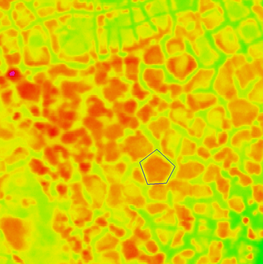
\includegraphics[width=9.5cm, height=8cm]{./figures/DEM_Area_B-HCP.png} \\
%\hspace*{0.8cm}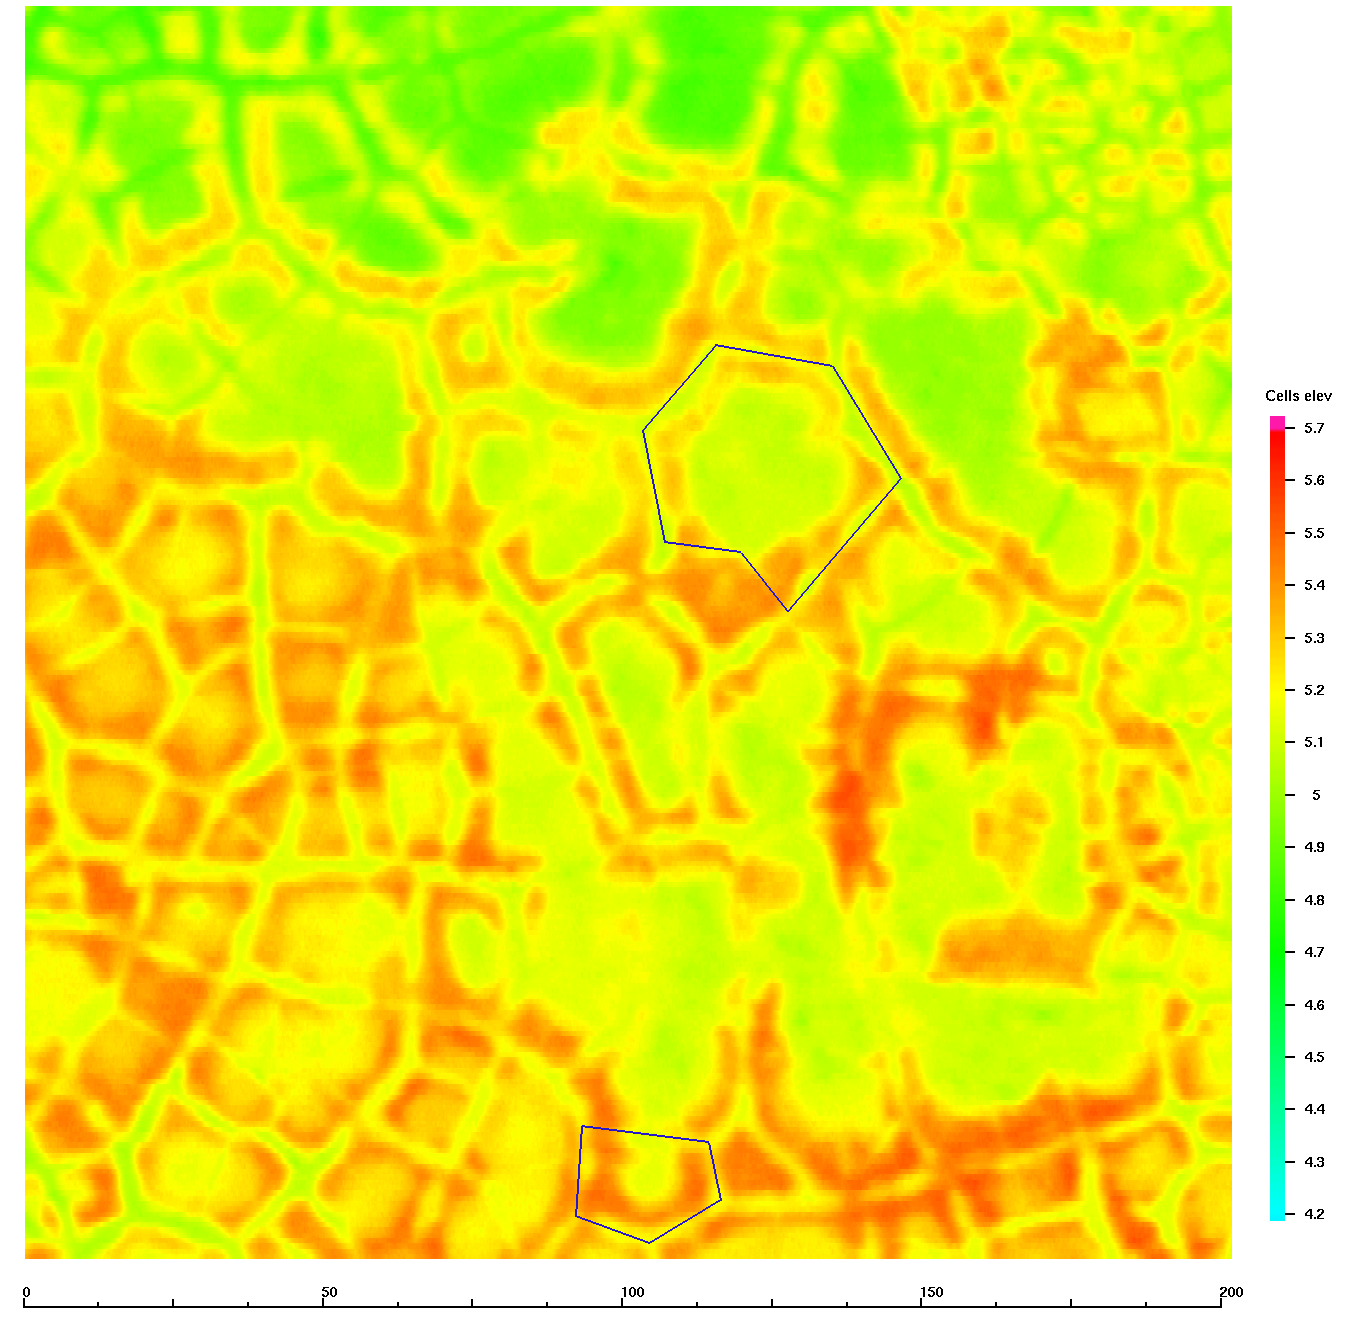
\includegraphics[width=10.8cm, height=8cm]{./figures/DEM_Area_A-LCP.png}
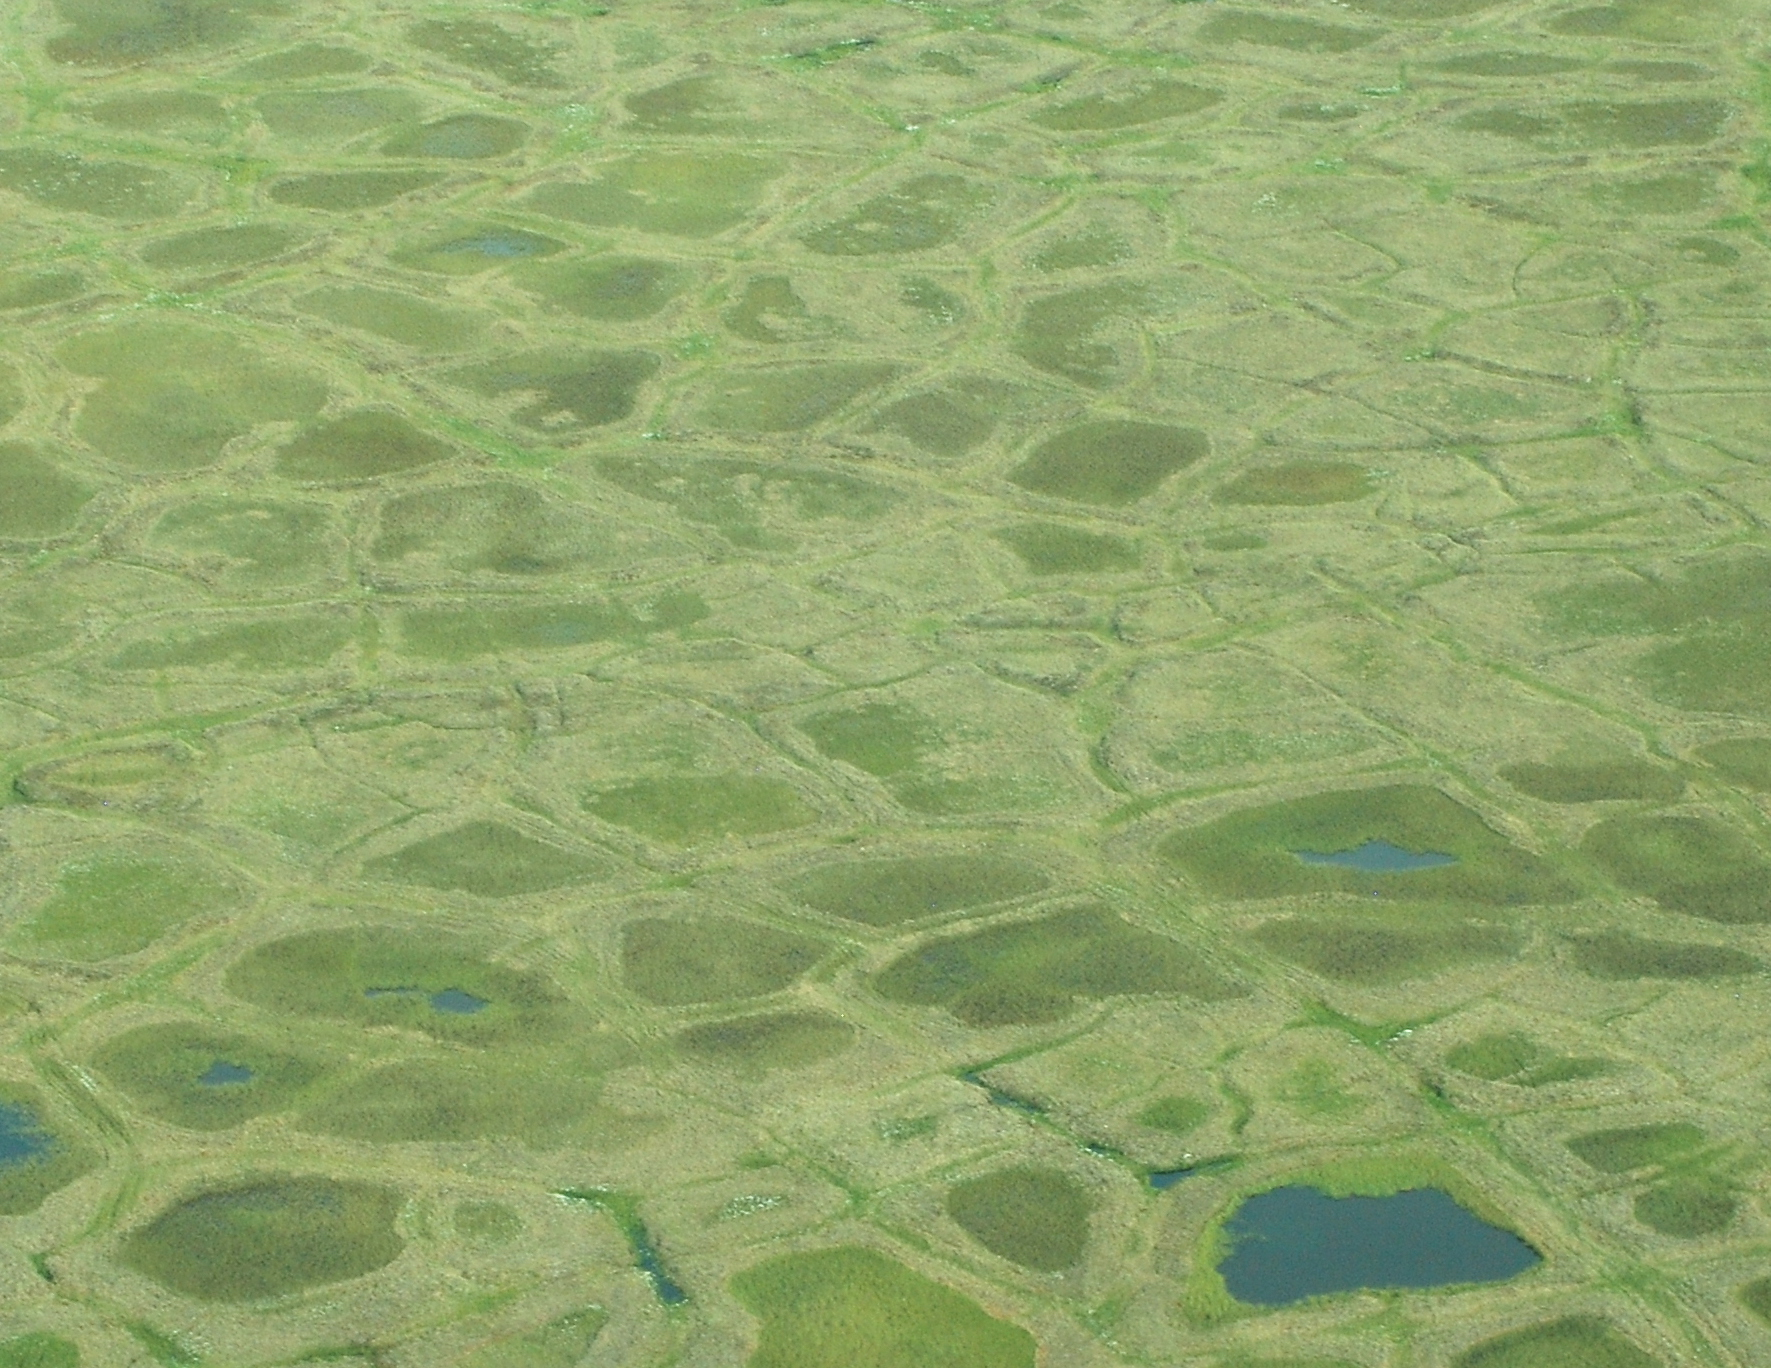
\includegraphics[width=9.5cm, height=8cm]{./figures/polygonal-landscape.jpg}
\caption{An illustration of a patterned polygonal tundra landscape within Barrow Environmental Obervatory near Alaska (courtesy of Stan D. Wullschleger).}
%\caption{An illustration of a patterned polygonal tundra landscape characterized by high-centered (top) and low-centered (bottom) polygons, located at NGEE-Arctic field sites A and B within Barrow Environmental Observatory (BEO) near Alaska, see Figure~\ref{ngee-arctic-fieldsites}. Shown is surface elevation, with ... colors representing higher elevations}
\label{tundra-sitesA-B}
\end{figure}
%

Here we present a subgrid parametrization for microtopography within macroscale surface flow simulations, and test the hypothesis that the effects of microtopography can be captured in coarsened models through the use of a subgrid model.
Our motivation for the new subgrid model is for use in a recently developed efficient and scalable mixed-dimensional model~\citet{jan2017} for integrated  surface/subsurface thermal hydrology in permafrost-affected landscapes, although we only address surface flow here.  
While polygonal tundra is the motivating application, the approaches used here are likely applicable in a more general context. 
%

Though the concept of including microtopographic features and their implications on flow and discharge is not new, it has not been fully addressed and understood from a modeling perspective. 
In the mid-1950s, the significance of the surface microtopographic features were described~\citet{stammers1956effect}. 
Panday and Huyakorn (\citetyear{panday2004fully}) presented an integrated surface/subsurface flow model with a subgrid representation that modified the overland flow governing equation to represent the effects of depressions and obstructions. 
One-dimensional simulations to study the effects of spatially varying surface roughness on flow hydrographs is presented by Huang and Lee~(\citetyear{huang2009influences}). Sally et al.(~\citetyear{thompson2010role}) analyzed the role of microtopography on partitioning rainfall into runoff and precipitation. They have shown an increase of 20-200$\%$ in the infiltration as compared to sheet-flow in 1-D hillslope simulations. 
In a numerical experiment at a scale of a few meters, Frei et al.~(\citetyear{frei2012surface}) highlighted that surface microtopography in wetlands can lead to the formation of biogeochemical hot spots. 
Frei and Fleckenstein~(\citetyear{frei2014representing}) use a spatially varying rill/depression storage concept to account for microtopographic effects in plot scale simulations for integrated surface/surface flow. 
%

Our subgrid approach is similar to the framework proposed by Panday and Huyakorn (\citetyear{panday2004fully}). We extend their approach by fully specifying a strategy for determining all of the needed parameters and equations and evaluating the subgrid parameterization with fine-scale simulations.
Several of these parameters may be extracted from a highly resolved digital elevation model (DEM) representing surface microtopography for single ice-wedge polygons.
Others are less straightforward, and we evaluate three methods for determining these with the goal of finding a strategy that is appropriate for large-scale simulations.
First we calibrate these parameters on single-polygon simulations, leveraging the ability to quickly solve a fine-scale problem on such a small domain.
Next we evaluate a geometric strategy based on percolation theory, and show that the parameters predicted by this method are well-correlated with the calibrated values.
Neither of these strategies are practical for landscape-scale simulations, as this would require thousands of polygons to be delineated (typically by hand) and analyzed.
This leads us to develop an alternate strategy in which we select parameters based solely on classification into low-, intermediate-, and high-centered polygons and use typical values for each class, which provides the opportunity to scale to large polygonal tundra landscapes.
This strategy is then evaluated on a cluster of polygons to evaluate the value of the subgrid model in improving hydrographs and surface storage.

This manuscript is organized as follows. 
Section~\ref{field-site} introduces the Arctic patterned polygonal ground, and discusses the role of microtopography. 
Section~\ref{surf-flow-system} presents the governing equations of the surface flow without a subgrid model, then motivates a subgrid model for changes in surface storage and lateral fluxes due to depressions and obstructions. 
In Section~\ref{numerical-tests} we evaluate the model.  
First we select seven polygons representative of a variety of types of polygons, and perform both fine and coarse-scale simulations.
The geometric model is evaluated, and calibrations are performed to improve the fit of hydrographs.
These results, shown in Section~\ref{numerical-tests-single}, demonstrate that a subgrid model can be used in coarse-scale models to improve characterization of the hydrologic function of a polygon.
In Section~\ref{numerical-tests-cluster}, we then look to evaluate the model on simulations which are more typical of the desired landscape scale results.  
Multiple polygons are simulated under the assumption that parameters cannot be directly calculated for each polygon.
We compare simulation results using our subgrid model to those from both fine-scale and coarse-scale (without a subgrid model) simulations to show that the subgrid model improves the ability of a coarse-scale model to predict hydrologic function in polygonal ground. 
Finally, in Section~\ref{conclusion}, we offer closing remarks and future research directions. 


\section{Field Site: Arctic Patterned Polygonal Ground}\label{field-site}
A large amount of frozen organic carbon is stored in permafrost-affected soils of the Northern Hemisphere~\citet{schuur2015climate,bg-11-6573-2014}.
The ground in Arctic regions is temperature-sensitive and under potential risk of carbon release to the atmosphere in a changing climate~\citet{hinzman2005evidence}.
Arctic landscapes often exhibit polygonal patterned (interconnected polygons approximately 10-20 m in diameter) ground.
The formation of polygonal landscapes in permafrost-affected regions is a consequence of freeze/thaw cycles over hundreds or thousands of years.
During winter, vertical fractures are formed due to ground contraction. In the spring, water from the snowmelt penetrates those cracks and refreezes.
The expansion of the ice in the cracks compresses the soil horizontally.
The recurring crack-compression process over long periods of time results in wedges of ice that honeycomb the subsurface and express as polygonal patterns on the surface~\citet{lachenbruch1962mechanics,greene1963contraction,mackay1990some,mackay2004thermally}.
Figure~\ref{ngee-arctic-fieldsites} shows an example~\citet{kumar2016modeling} of polygonal tundra from the Barrow Environmental Observatory (BEO), a field site of the U.S. Department of Energy's Next Generation Ecosystem Experiments (NGEE) Arctic project.
%
\begin{figure}[!h]
\centering
 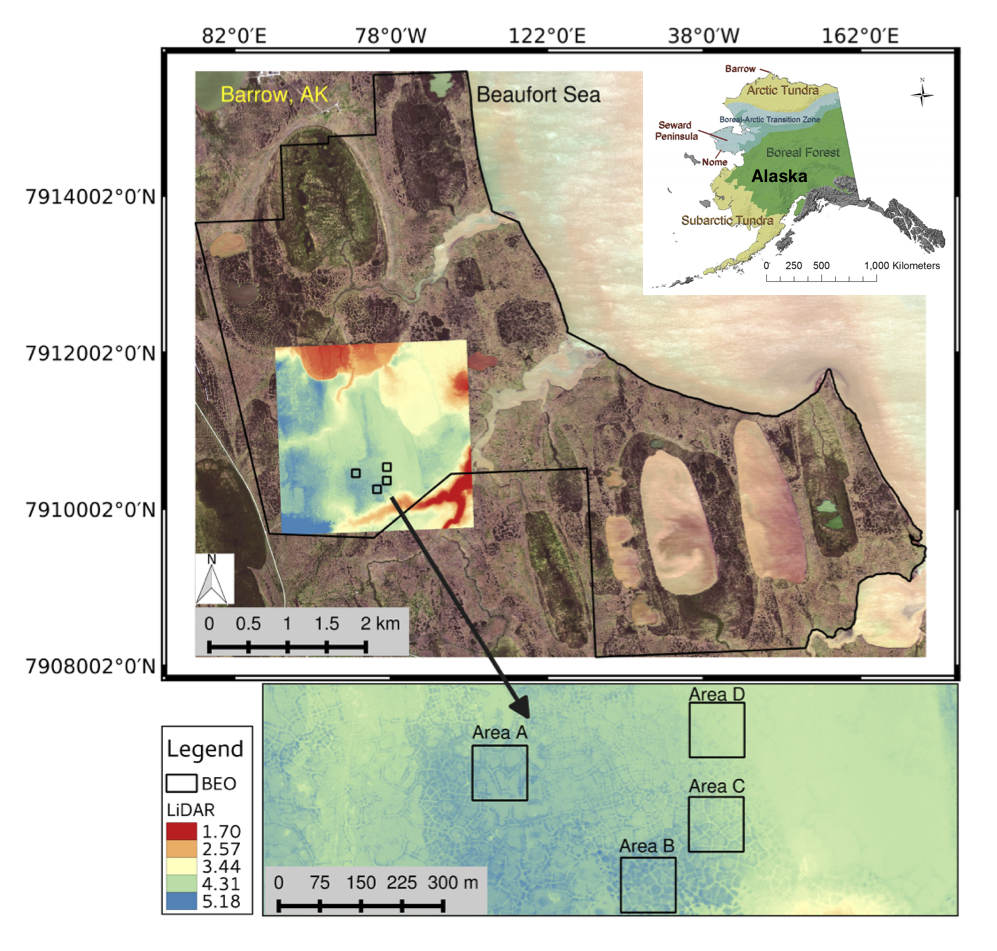
\includegraphics[width=14cm, height=17cm]{./figures/ngee-arctic-fieldsites.png}
\caption{NGEE-Arctic field sites at the BEO. Image adapted from~\citet{kumar2016modeling}.}
\label{ngee-arctic-fieldsites}
\end{figure}
%

Ice-wedge polygons are often classified as low-centered polygons (LCPs) or high-centered polygons (HCPs) based on surface microtopography.
The typical LCP has a raised rim and central depression, and thereby holds ponded water in the center during the summer that can only be available for infiltration and evaporation.
The typical HCP has an elevated center that slopes downward to the trough, stores less water and increases runoff as compared to the LCPs. 
Thawing of ice-wedges in a warming climate causes the raised rims of LCPs to subside leading to the formation of HCPs~\citet{jorgenson2006abrupt}.
The evolution of LCPs to HCPs has the ability to connect the disconnected troughs, and thus transform a poorly drained tundra to a well-established drainage network.
This trough-rim-center microtopography change occurs along a scale of centimeters to a few meters, but potentially alters the entire ecosystem and brings substantial hydrological changes (e.g., surface/subsurface interactions, distribution of surface water, discharge rate etc.)~\citet{liljedahl2016pan, hinzman2005evidence,rowland2010arctic,liljedahl2012ice}.

\FloatBarrier

%
% Section: Surface Flow Model
% ================================================================================
\section{Surface Flow Model}\label{surf-flow-system}
This section describes an extension of the diffusion wave equation for surface flow to incorporate the effects of surface microtopography in coarsened models.

%
% Subsection: surface flow
% ----------------------------------------------------------------------
\subsection{Surface flow without subgrid scale information}
The evolution of surface water is governed by conservation of water and a water flow law.
Here, as is typical, we measure the extent of water in volumetric units, i.e. m$^3$ water per m$^2$ surface area, or simply meters of water hereafter.
Then, conservation is described by:
%
\begin{equation}\label{diffwaveeq}
\frac{\partial \delta}{\partial t} + \nabla \cdot q = q_\text{rp} + \Gamma_\text{ex},
\end{equation}
%
where $\delta$ represents ponded depth [m], $q_\text{rp}$ is the rain precipitation rate [m / s], $\Gamma_\text{ex}$ is water exchange between surface and subsurface systems [m / s], $t$ is time [s], and $q$ denotes surface volumetric flux [m$^2$ / s].
The volumetric flux of water is approximated using a diffusion wave equation which multiplies the fluid parcel velocity $U$ by the flowing cross sectional area (per unit edge length):
%
\begin{align}
\label{diffwaveeq_flowlaw}
q &= \delta U \nonumber\\
  &= \delta \left[ -\frac{\delta^{2/3}}{n_\text{mann} (\| \nabla z\| +\epsilon)^{1/2}} \nabla(z + \delta) \right]
\end{align}
%
where $n_\text{mann}$ is Manning's coefficient [m$^{-1/3}$ s)], $z$ is surface elevation [m], and $\epsilon >0$ is a regularization parameter used to avoid zero bed slope.
More details about the implementation of this model  can be found in~\citet{spainter2016integrated}. 

%
% meshes
% ----------------------------------------------------------------------
\subsection{A Coarsening Strategy based on Polygons}
As discussed in Section \ref{field-site}, microtopography on the scale of a meter must be resolved in order to capture the effect of topography change.
Therefore we consider a ``fine-scale'' mesh, $\Omega_z$, whose surface topography $z(x,y)$ [m] is presumed given by a DEM.
We look to coarsen this onto a ``coarse-scale'' mesh, $\Omega_{\bar{z}}$ with topography $\bar{z}(x,y)$, in which each cell of the mesh coincides with a polygon tracing the troughs.
Elevations of these polygons at the coarse-scale are determined from the same DEM.
Then we define microtopography as the component of the topography on polygon $A$ not captured in the coarse-scale mesh:
%
\begin{equation}\label{local_topography}
  Z = z - \bar{z}.
\end{equation}
%
We note that the surface $\bar{z}$ within the polygon may not be planar; we approximate it as the best fit plane to the coarse mesh.
This splits the topography between long wavelength topography which is captured by the coarse-scale mesh and short wavelength topography (or microtopography), whose effect is to be captured by a subgrid model.

%
% subection subgrid model
% ----------------------------------------------------------------------
\subsection{Subgrid Model}\label{subgridmodel}
Most subgrid models, including this one, look to represent microtopography as depressions and obstructions.
These are addressed by altering the accumulation of water (the time derivative in equation \ref{diffwaveeq}) and the flow law, equation \ref{diffwaveeq_flowlaw}, resulting in a model of the form:
%
\begin{equation}\label{subgrid}
\frac{\partial \Phi (\delta)}{\partial t} + \nabla \cdot q_s = q_\text{rp} + \Gamma_\text{ex}.
\end{equation}
%
This differs from equations \ref{diffwaveeq}-\ref{diffwaveeq_flowlaw} through the introduction of a volumetric depth $\Phi(\delta)$ [m] and an effective volumetric flux $q_s$ [m$^2$ / s] to account for subgrid depressions and obstructions.
A volumetric depth is introduced to account for the fact that the same volume of water, on rough topography, reaches a different height than that on a flat surface.
An effective velocity is introduced to capture two observations: depression storage and flow path obstructions.
On a rough surface, small amounts of water may not flow at all if there are depressions in which that water ponds.
And if protrusions keep water from flowing in sheet flow across the cell, then it may have to divert around those obstructions, resulting in longer time to cross the cell, and therefore slower effective velocities.

We note that this conceptual model structure is typical in the literature; it was proposed by \citet{stammers1956effect,mwendera1992estimation}, and adopted by others including \citet{panday2004fully,thompson2010role,frei2012surface,frei2014representing}.
Where models differ is in how they derive, calibrate, or specify these altered quantities; here we propose a model whose parameters may be estimated in a few different, independent ways, and compare the predicted results with the ``truth'' calculated from a fine scale model.

\subsubsection{Derivation of Volumetric Depth}
First we look to relate the volume of water (per unit area) to the height of the free surface.
On a flat cell with no subgrid topography, this volume is given simply by the height of the free surface.
On a rough cell, this is not the case, but the volumetric depth may be calculated on geometric arguments.
Specifically, if the microtopography on a coarse-grid cell $A$ of area $|A|$ is given by $Z(x,y)$, with minimum elevation $Z_\text{min}$, then the volume of water (per unit area) is given by:
%
\begin{equation}\label{volumetric-depth1}
\Phi (\delta) = \frac{1}{|A|} \int_A \left( \delta + Z_\text{min} - Z(x,y) \right ) \mathcal{H} \left( \delta + Z_\text{min} - Z(x,y) \right ),
\end{equation}
%
where $\mathcal{H}$ is the Heaviside function.
This could be computed directly from the microtopography for a given $\delta$, but this would require a complex workflow to do in practice.
Alternatively for each polygon, we employ a simpler parameterization, characterized by two parameters: (1) the elevation range spanned by the subgrid microtopography $\Delta_\text{max} \equiv Z_\text{max} - Z_\text{min}$, where $Z_\text{max}$ is the maximum elevation, and (2) the total excluded volume, given by:
%
\begin{equation}\label{volumetric-depth1b}
\Delta_\text{exc} \equiv \frac{1}{|A|} \int_A \left( Z(x,y) - Z_\text{min} \right ).
\end{equation}
%
It is clear that, once $\delta > \Delta_\text{max}$, there is no more soil excluding volume, and so the volume is given by $\delta - \Delta_\text{exc}.$
Expanding a cubic polynomial in $\frac{\delta}{\Delta_\text{max}}$, ensuring that the volumetric depth must be $0$ at $\delta = 0$, noting from direct geometric computations that the derivative is also typically $0$ at $\delta = 0$, and requiring that both the value and derivative are continuous at $\delta = \Delta_\text{max}$ suggests the following empirical model of volumetric depth:
%
\begin{equation}\label{volumetric-depth2}
\Phi (\delta) =
\begin{cases} (2 \Delta_\text{max} - 3 \Delta_\text{exc}) \left(\frac{\delta}{\Delta_\text{max}} \right )^2 + (2 \Delta_\text{exc} -  \Delta_\text{max}) \left(\frac{\delta}{\Delta_\text{max}} \right )^3 & \text{if} \hskip 0.1in 0 \leq \delta \leq \Delta_\text{max}, \\
\delta - \Delta_\text{exc} & \text{if} \hskip .1in \delta > \Delta_\text{max}.
\end{cases}
\end{equation}
%

The volumetric depth calculated from the parameterization in Equation~\ref{volumetric-depth2} (curve) is compared with the direct calculation in Equation~\ref{volumetric-depth1} (dots) for two selected ice-wedge polygons in Figure~\ref{volumetric-depth-fig1} (HCP (left) and LCP (right)).
These fits are typical of seven polygons discussed below.
Also shown is the volumetric depth in the absence of microtopography, which is linear with slope unity.
Equation~\ref{volumetric-depth2} is an appropriate parameterization for polygonal ground, and may or may not be for other microtopographic features.
%
\begin{figure}[!h]
\centering
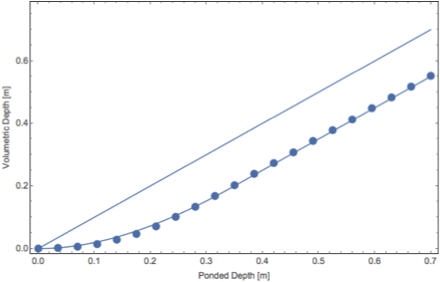
\includegraphics[width=6cm, height=6cm]{./figures/polygons-finescale/picture2.png} % A01- HCP
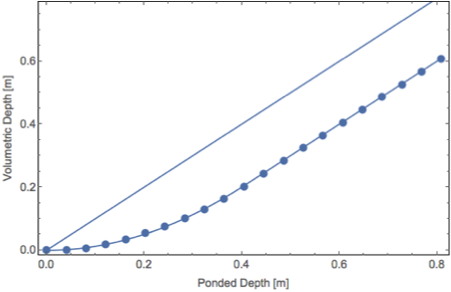
\includegraphics[width=6cm, height=6cm]{./figures/polygons-finescale/picture3.png} %B01-LCP
%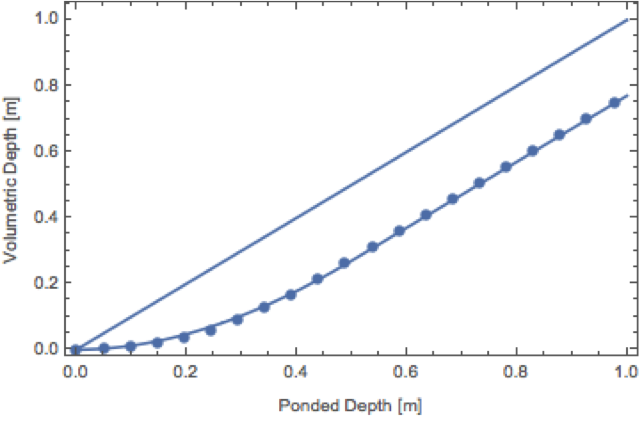
\includegraphics[width=6cm, height=6cm]{./figures/polygons-finescale/polygon40.png}
%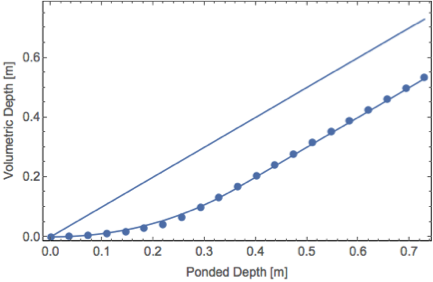
\includegraphics[width=6cm, height=6cm]{./figures/polygons-finescale/picture4.png}
%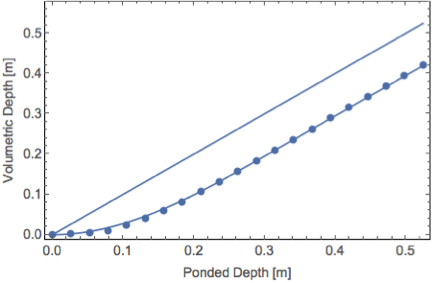
\includegraphics[width=6cm, height=6cm]{./figures/polygons-finescale/picture5.png}
\caption{Volumetric depth versus ponded depth for two selected ice-wedge polygons. The ice-wedge polygons are displayed in Figure~\ref{IWP-finemesh}. Left: high-centered polygon. Right: Low-centered polygon.}
\label{volumetric-depth-fig1}
\end{figure}

\subsubsection{A Modified Flow Law}
Microtopographic effects on the flow law are not as straightforward to incorporate as the volumetric head.
We make the distinction between depressions and obstructions.
Depressions are disconnected low points in the topography that the ponded depth must rise above before any flow can happen.
Obstructions exist above the depressions and interrupt and slow the flow, but do not block it completely.
To model the effects of obstructions and depressions, we propose the following modified form of the volumetric flux:
%
\begin{align}
\label{modified-velocity}
q_s &= \left( \Phi(\delta) - \Phi(\delta_\text{d}) \right) U \nonumber \\
    &= \left( \Phi(\delta) - \Phi(\delta_\text{d}) \right)\left[- \left(\frac{\left( \Phi(\delta) - \Phi(\delta_\text{d}) \right)}{\delta - \delta_\text{d}}\right)^\beta \frac{ \left[ \mathcal{H} \left( \delta - \delta_\text{d}\right )\left(\delta - \delta_\text{d}\right)\right]^{2/3} }{n_\text{mann} (\| \nabla Z \| +\epsilon)^{1/2}} \nabla(Z + \delta) \right],
\end{align}
%
where $\delta_\text{d}$ is a depression depth [m] that measures the height at which water overtops all depressions resulting in a connected pathway of ponded water between inlet and outlet, and $\beta$ is a tunable exponent which controls how much drag obstructions provide (larger values yield slower rising and falling limbs in hydrographs).
Here Manning's equation is altered in three ways, from left to right in appearance:
%
\begin{itemize}
\item $\Phi(\delta) - \Phi(\delta_\text{d})$ replaces $\delta$ as the flowing cross sectional area (per unit edge length).
\item An obstruction drag factor, $\left(\frac{\left( \Phi(\delta) - \Phi(\delta_\text{d}) \right)}{\delta - \delta_\text{d}}\right)^\beta$ is included that captures the effect of obstructions slowing down the fluid velocity, but approaches $1$ for $\delta \gg \delta_\text{d}$.
\item $\delta - \delta_\text{d}$ is used instead of $\delta$ for the conductivity, ensuring that no flow from depressions is allowed.
\end{itemize}
%
It is straightforward to confirm that, independent of $\beta$, the following physical limits are captured:
%
\begin{itemize}
\item For no water, i.e. $\delta = 0$, $U$ is zero.
\item For large amounts of water or small topography, where $\delta \gg \Delta_\text{max}, \Phi(\delta) = \delta - \Delta_\text{exc} \approx \delta$ and $\delta - \delta_\text{d} \approx \delta$, and equation \ref{modified-velocity} reduces to the standard diffusion wave equation \ref{diffwaveeq_flowlaw}.
\item In the case of depressions but no obstructions, i.e. $\Delta_\text{max} = \delta_\text{d}$, then the equation results in no flow until depressions are filled, after which flow is given by the standard diffusion wave equation above the (filled) depressions.
\item In the case of obstructions but no depressions, i.e. $\delta_\text{d} = 0,$ there is no delay in flow, but both velocity and flux are reduced by an obstructed fraction.\end{itemize}
%
It remains then to specify how $\delta_\text{d}$ and $\beta$ are determined.
Qualitatively, larger depression depth results in larger delays in the onset of runoff, while larger $\beta$ results in smaller slopes of the rising and falling limbs of a hydrograph.

%% \ethan{Not sure this paragraph adds value --etc}
%% Note that this quantity is nontrivial, and may actually be dependent upon the flow regime.
%% For instance, consider the depression of a low-centered polygon, i.e. polygon A01 in Figure \ref{IWP-finemesh}.
%% For a simulation of snowmelt, the polygon center is an active depression, and must fill before snow melting in the polygon center can run off.
%% For a simulation of inundation, the polygon center is an excluded depression, as flow may move through the troughs and around the center without filling that depression.
%% Therefore we consider a variety of strategies for specifying depression storage, and note that the best choice may actually be problem dependent.

In summary, we hypothesize that the microtopographic effects on surface flow can be captured with a simple approximation with four parameters:
%
\begin{itemize}
\item subgrid relief $\Delta_\text{max} = Z_\text{max} -   Z_\text{min}$, where  $Z_\text{max}$ and  $Z_\text{min}$ are the maximum and minimum elevation in the microtopography,
\item specific excluded volume $\Delta_\text{exc}$, the soil volume above the microtopographic low point normalized by IWP area,
\item depression depth $\delta_\text{d}$, a measure of how much water must first fill depressions before flow can span the polygon, and
\item obstruction drag exponent $\beta$, a measure of how much obstructions slow the flow.
\end{itemize}
%
The subgrid relief and specific excluded volume can be computed directly from the microtopography (univariate statistics), while the depression depth and drag exponent will be investigated in numerical experiments below.

%
% subsection: implementation
% ----------------------------------------------------------------------
\subsection{The Advanced Terrestrial Simulator (ATS)}\label{ATS}
This subgrid model has been implemented in the Advanced Terrestrial Simulations (ATS).
The ATS is an open source code~\citet{ats-website} and has the capabilities to simulate fully integrated surface/subsurface soil thermal hydrology with modeling of snow distribution and surface energy balance~\citet{spainter2016integrated, atchley2015}.
The underlying framework of the ATS builds on Amanzi (a flow and reactive transport simulator, see~\citet{moulton2012high}), and is based on a multiphysics management tool called Arcos~\citet{ecoon2016managing}.
Arcos provides a strategy for easily implementing and coupling new physics capability; our subgrid model, which reuses significant parts of a standard diffusion wave implementation, but substitutes in new model evaluators such as conductivities and volumetric depth, leverages this capability.
As a result, these models can be quickly developed and tested, and are coupled to existing capability within ATS.


%
% Section: Results
% ================================================================================
\section{Numerical Results and Discussions}\label{numerical-tests}
\FloatBarrier

In this work, we will be referring to three types of models as follows:
%
\begin{description}\itemsep0pt \parskip0pt
\item I. \emph{Fine-scale model:} Diffusion wave equation with a microtopography-resolving unstructured mesh $\Omega_z$ (cells on order of 0.1 m in diameter). 
\item II. \emph{No subgrid model:} Diffusion wave equation with coarsened unstructured mesh $\Omega_{\bar{z}}$, where each mesh cell corresponds to an ice-wedge polygon (cells on order of 20 m in diameter).
\item III. \emph{Subgrid model:} Modified diffusion wave equation (derived in subsection~\ref{subgridmodel}) on $\Omega_{\bar{z}}$
  \begin{description}
  \item S$_1$) Individually calibrated model parameters
  \item S$_2$) Geometrically determined model parameters
  \item S$_3$) Lumped model parameters by polygon type
  \end{description}
\end{description}
%
Model I provides the ``true'' solution, in the sense that our goal is to represent this solution faithfully using a coarse-scale model.
Model II provides the ``control'' simulation, in the sense that this is the scale assumed to be computationally feasible to simulate over large landscapes.
Our goal is to investigate whether and how subgrid models can improve a simulation at the scale of Model II to capture some information from Model I.
We do not expect to fully match Model I, but instead look to include some of the key aspects of the simulation, such as effective breakthrough times, rising and falling limbs, etc.

In Model III, we consider multiple strategies for specifying the depression depth $\delta_\text{d}$ and obstruction drag exponent $\beta$.
First, we perform hand-calibrated simulations on seven individual polygons, in which $\delta_\text{d}$ and $\beta$ are chosen so as to best fit the fine scale simulations.
This approach is intended to ensure that the model \emph{can} reasonably improve the ability of coarse-scale models to represent fine-scale microtopography.
While this results in an excellent fit, we note that this is not the end goal, as calibrating each and every individual polygon at the landscape scale is likely not possible from a workflow perspective.
Next we consider a purely geometric approach based on site percolation.
Specifically, we fill the lowest elevation surface cells until the cluster of inundated cells forms a connected backbone spanning the polygon.
While the geometic predictions themselves do not result in good fits, they are well-correlated with the calibrated values, suggesting a strategy in which this empirical correlation is used to run percolation algorithms on every polygon, then leverage the correlation to generate reasonable paramters.

However, for a landscape scale capability, we wish to avoid individually analyzing every polygon.
As each of the other parameters are easily characterized, it is straightforward to generate landscapes of statistically reasonable polygons, given a strategy for choosing depression depths and obstruction drag exponents.
Toward this goal, the calibrated parameters are lumped by their polygon type (high-, intermediate-, and low-centered polygons), generating a ``typical'' value for each type of polygon.
This is a viable strategy for larger scales, since classification algorithms have been shown to be accurate when based upon arial or satelite imagery \citet{Skurikhin2013}.


%
% Section: Results -- single IWP
% --------------------------------------------------------------------
\FloatBarrier
\subsection{Single ice-wedge polygons}\label{numerical-tests-single}

We consider seven individual ice-wedge polygons (IWPs) (Figure~\ref{IWP-finemesh}) from the Barrow Environmental Observatory (BEO).
The single ice-wedge polygons named A, B and C correspond to the NGEE Arctic field sites A, B and C (see Figure~\ref{ngee-arctic-fieldsites}), respectively, and polygons are numbered according to a manual polygon delineation.
Those polygons consist of low-centered (A polygons especially), high-centered (B polygons especially), and intermediate-centered polygons, each with well established troughs (relatively uniform elevation across the trough) and obstructions in the troughs, and hence represent a broader class of polygonal landscape.
Table~\ref{subgrid-parameters} displays subgrid parameters extracted from fine-scale topography of seven IWPs depicted in Figure~\ref{IWP-finemesh}.
%
\begin{center}
\begin{table}[htbp]
\caption{Parameters extracted from fine-scale microtopography for subgrid model. Top row corresponds to polygon type, and first column displays the extracted parameters.}\label{subgrid-parameters}
\begin{tabular}{| c |c|c|c|c|c|c|c|}
\hline
& C06 & C31 & C40 & C44 & C45 & A0 & B01 \\ \hline
 $\Delta_\text{max}(m)$ & 0.404 & 0.262 & 0.483 & 0.364 & 0.350 & 0.361 & 0.411 \\ \hline
$\Delta_\text{exc}(m)$ & 0.2 & 0.105 & 0.23 & 0.2 & 0.15 & 0.185 & 0.26\\ \hline
$ \delta_\text{d}(m)$ & 0.069 & 0.128 & 0.043 & 0.187 & 0.164 & 0.222 & 0.143 \\ \hline
\end{tabular}
\end{table}
\end{center}%

Numerical results presented in this subsection correspond to the two variants (S$_1$ and S$_2$).
A pulse numerical test (injection followed by recession) is performed: we start with a fully dry surface, and inject water at a constant rate at the inlet boundary until breakthrough happens (prescribed flux boundary for a certain period of time), then stop the water supply and let water pass through the outlet (free drainage boundary).
The inward and outward arrows shown in Figure~\ref{IWP-finemesh} indicate the inlet and outlet boundaries. 
In the coarsened cases, the elevation of faces depends on the elevation of the corners of the fine-scale IWP.
It is important to mention that the higher (inlet) and lower (outlet) boundaries are chosen based on the average elevation of the faces in the coarsened grid.
For instance, the inlet in the coarsened grid of the polygon A01 (shown in Figure~\ref{IWP-finemesh}) is higher than the outlet, however, the fine-scale inlet is, on average, lower than outlet. 
%
\begin{figure}[!h]
\centering
\vskip -2cm
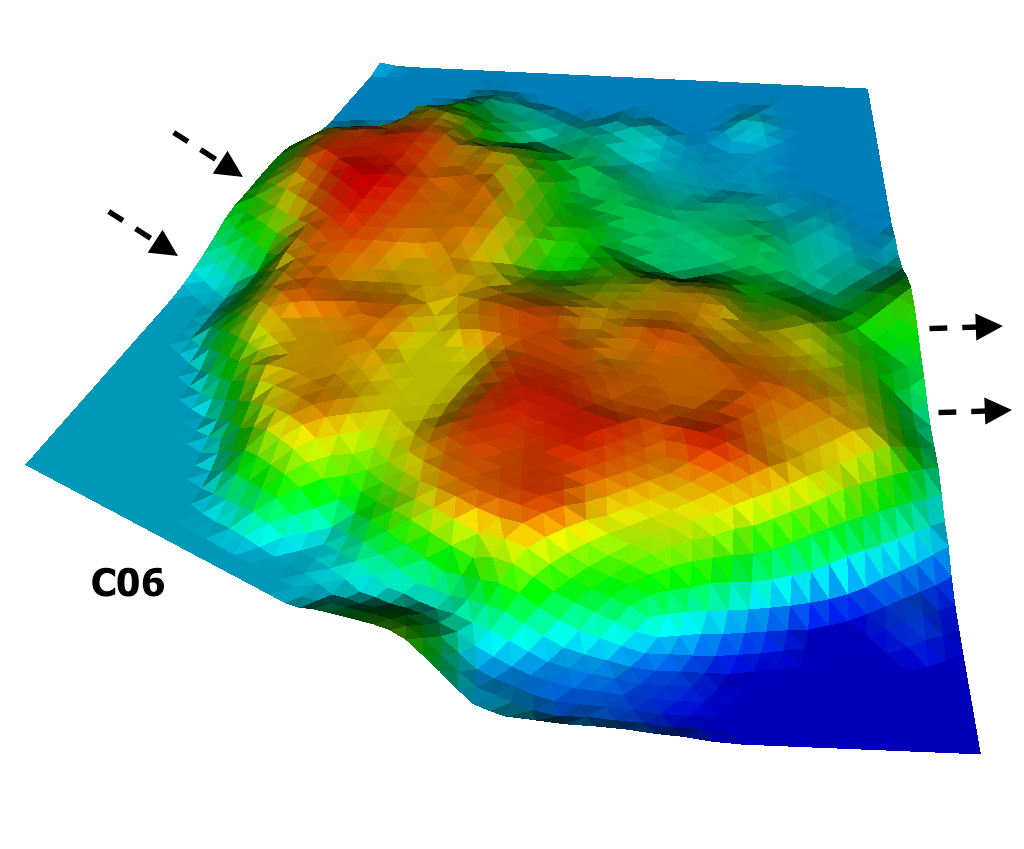
\includegraphics[width=6.2cm, height=3.5cm]{./figures/polygons-finescale/3Dpolygon06-3B.png}
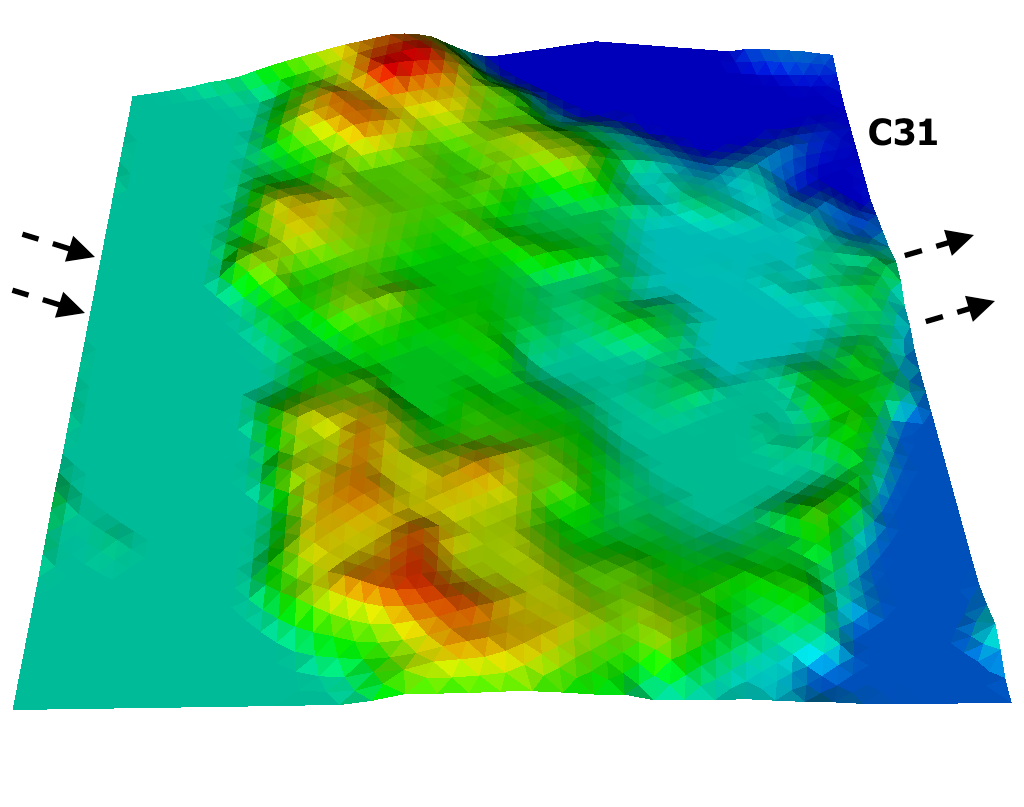
\includegraphics[width=6.2cm, height=3.5cm]{./figures/polygons-finescale/3Dpolygon31-3B.png}\\
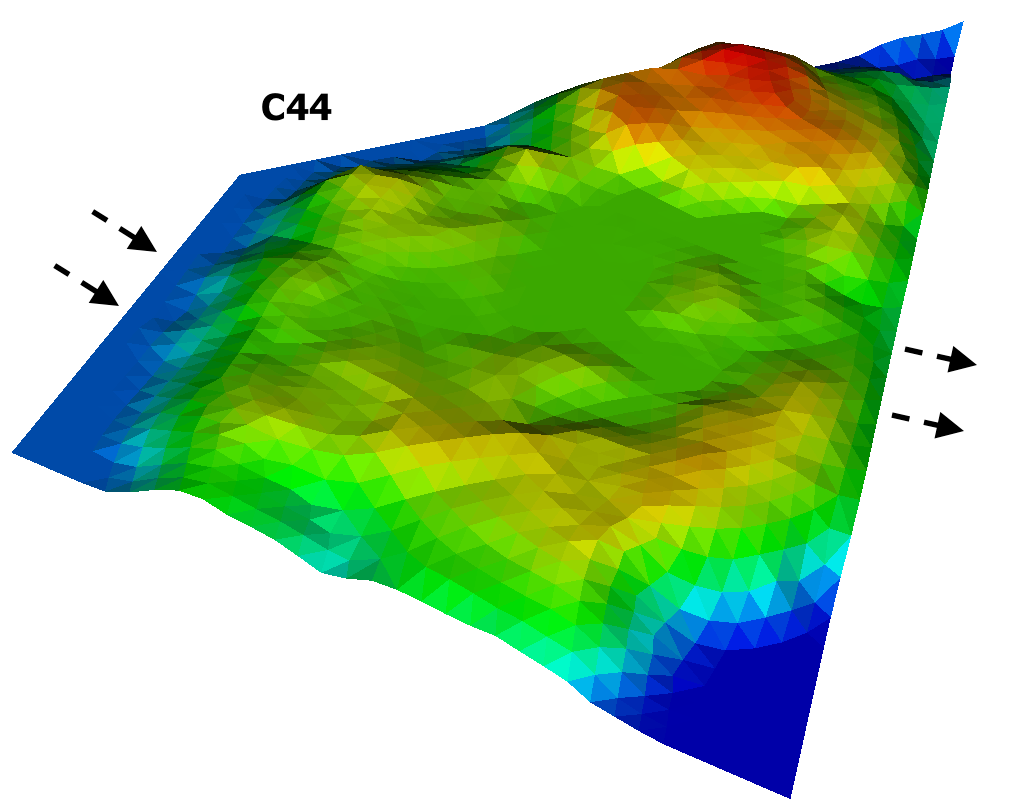
\includegraphics[width=6.cm, height=3.5cm]{./figures/polygons-finescale/3Dpolygon44-3B.png}
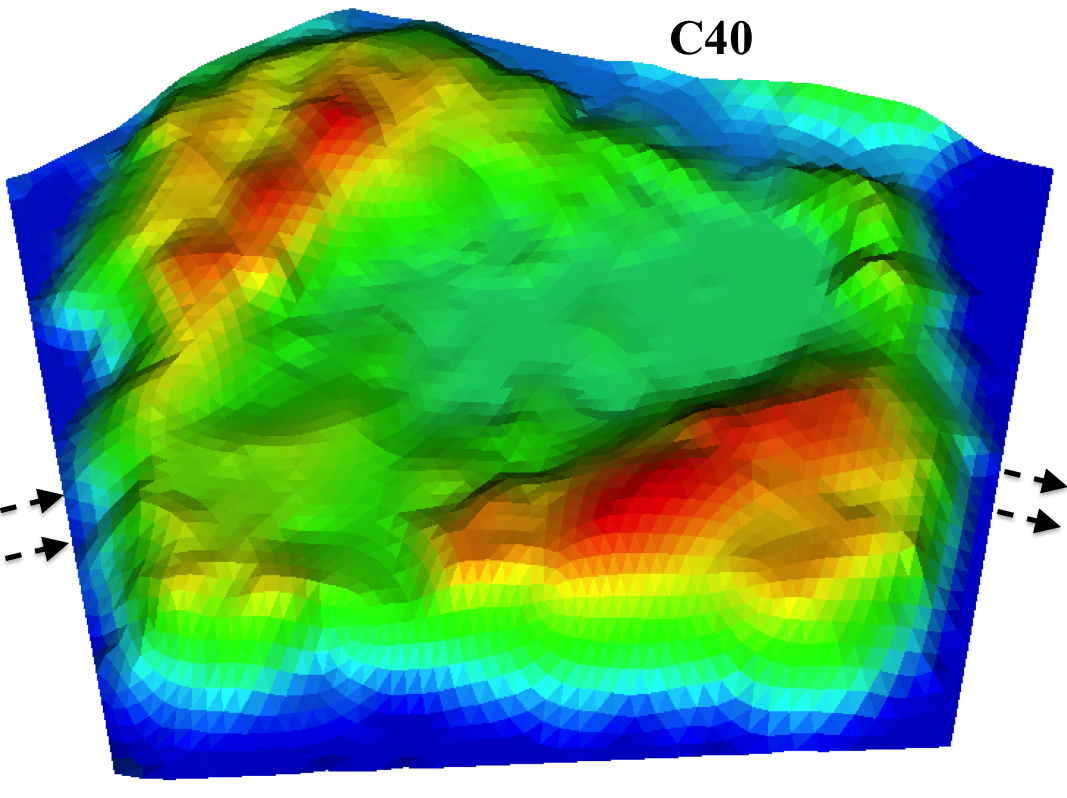
\includegraphics[width=6.2cm, height=3.5cm]{./figures/polygons-finescale/3Dpolygon40-1.png} \\
 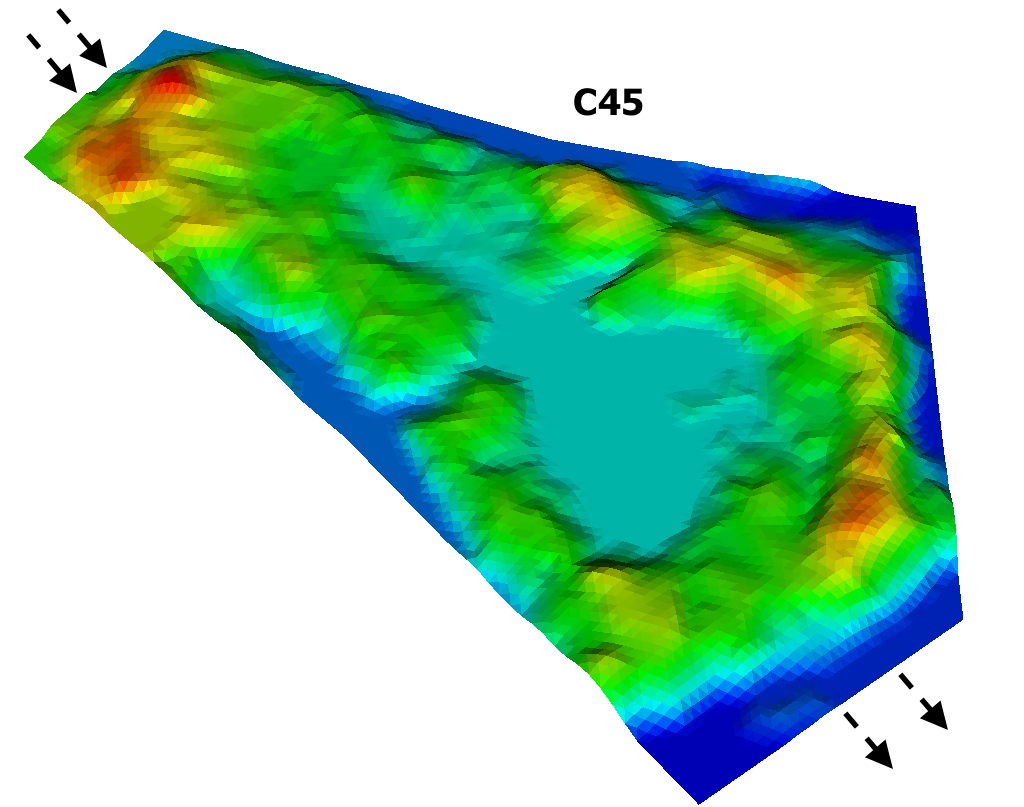
\includegraphics[width=6.2cm, height=3.5cm]{./figures/polygons-finescale/3Dpolygon45-3B.png}
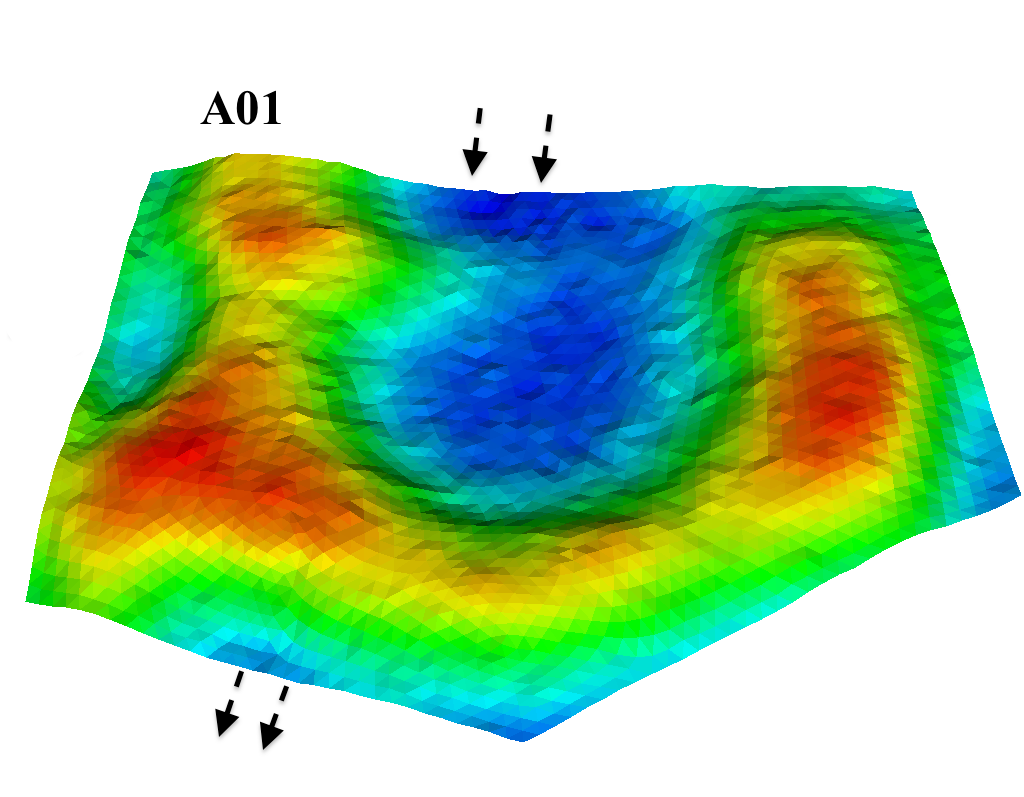
\includegraphics[width=6.2cm, height=3.5cm]{./figures/polygons-finescale/3DpolygonA01-3E.png}\\
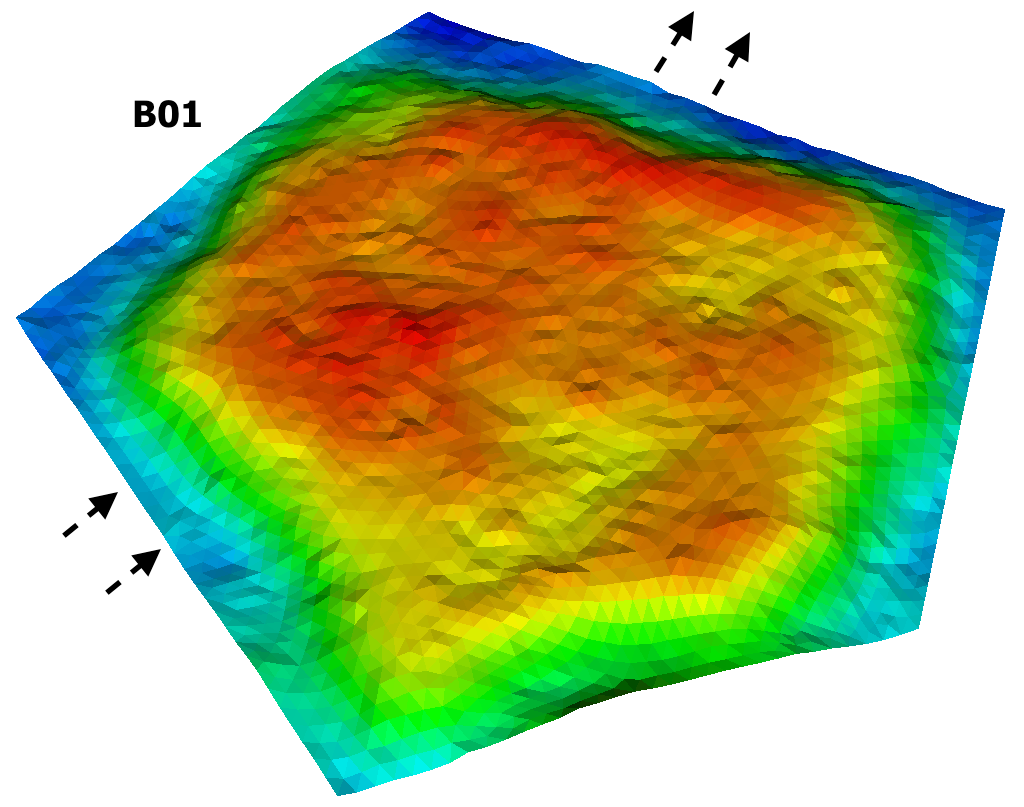
\includegraphics[width=6.2cm, height=3.5cm]{./figures/polygons-finescale/3DpolygonB01-3B.png} \\
\caption{An illustration of the microtopography of ice-wedge polygons from Barrow Environmental Observatory (BEO). Red and dark blue spots correspond to high- and low-elevated regions. The arrows indicate inlet and outlet boundaries. The choice of the inlet and outlet boundaries is  based on the higher and lower sides of the coarsened grid.}
\label{IWP-finemesh}
\end{figure}

\begin{figure}[!h]
\centering
\vskip -4.5cm
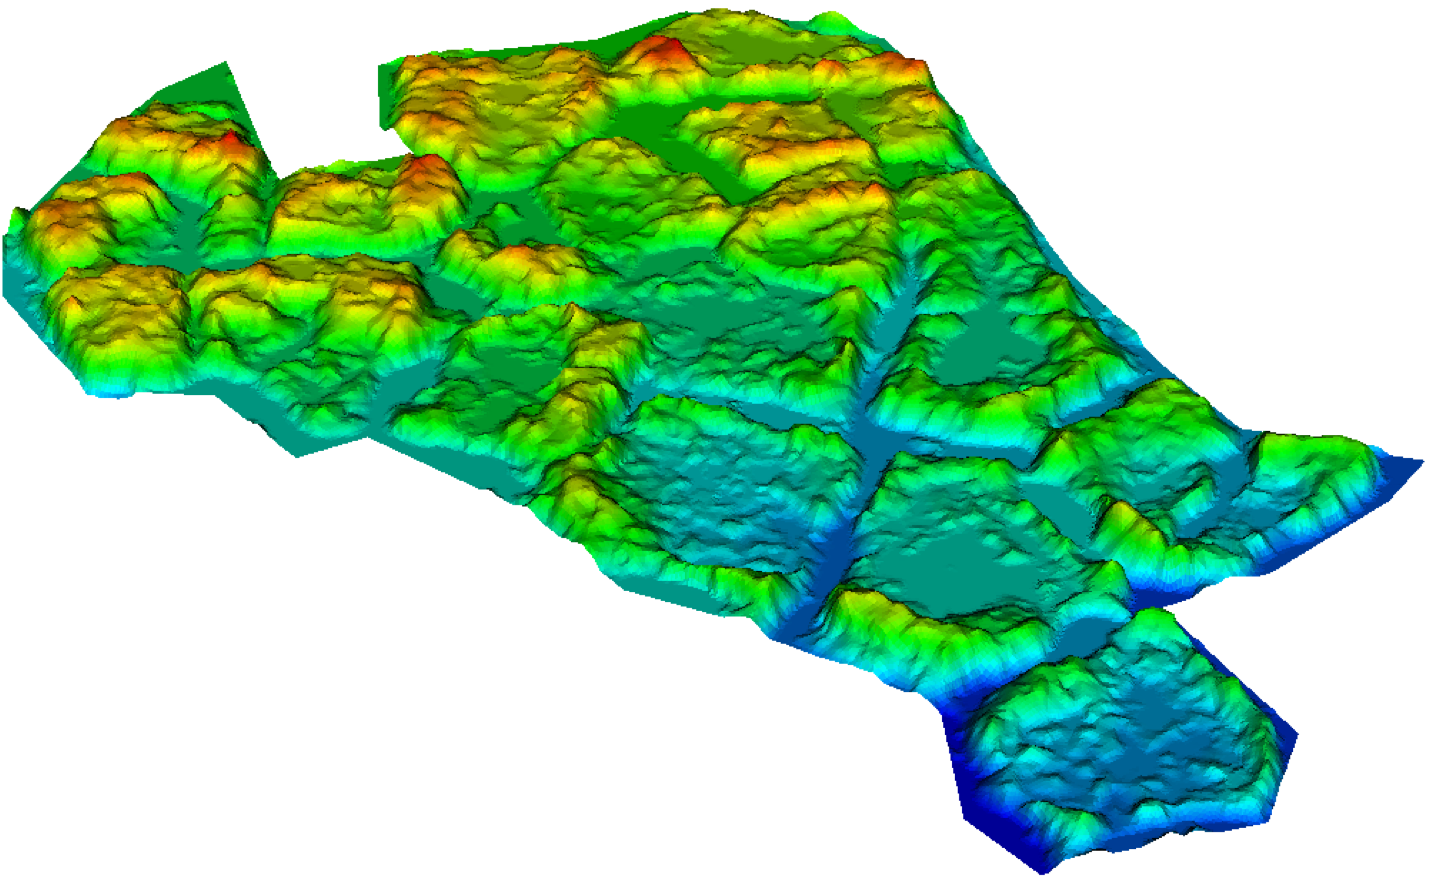
\includegraphics[width=12.2cm, height=6.5cm]{./figures/polygons-finescale/lobster-finemesh-elevation.png}
\caption{An illustration of the microtopography of a cluster of ice-wedge polygons from Barrow Environmental Observatory (BEO). Red and dark blue spots correspond to high- and low-elevated regions.}
\label{lobster-finemesh}
\end{figure}

We compare numerical results obtained in the variants S$_1$ and S$_2$ to those with the no-subgrid model and to fine-scale results on single IWPs. We have carried out detailed simulations on all the polygons shown in Figure~\ref{IWP-finemesh}, however, we discuss the results of polygon C44 in more detail; these results are representative of all the remaining polygons as far as the accuracy and shape of the hydrographs are concerned. 
Figure~\ref{polygon-C44} compares numerical results of the subgrid model with the fine-scale simulations, and no subgrid model of polygon C44. 
Clearly, Model III(S$_2$) fails to match the fine-scale simulations, delayed breakthrough (by 5 hours) in the subgrid model is an indication of higher depression depth computed by the percolation algorithm (see Figure~\ref{polygon-C44}a). 
Simulations with a calibrated depression depth, Model III(S$_1$) with $\beta = 1$, dramatically improves the shape of the hydrogragh and the water content in the system as shown in Figure~\ref{polygon-C44}b. 
However, a mismatch appears at the time of breakthrough and the beginning of recession period even with the use of a calibrated depression depth. 
As alluded to earlier, this is due to a large head gradient between the center and seepage face, and physically makes sense. 
Figure~\ref{polygon-C44}c illustrates the results of Study III(S$_1$) with $\beta = 3.0$.
Our subgrid model reproduces the fine-scale behavior, and the numerical results are nearly identical to the fine-scale simulations. 
However, a complete mismatch is observed in numerical results of the no-subgrid model. Early breakthrough and drier surface at the end of simulation are associated with no obstructions and depressions in the no-subgrid model. 
In contrast to the fine-scale and subgrid models, as long as the head gradient is sufficient the drainage continues at the outlet.


\begin{figure}
\centering
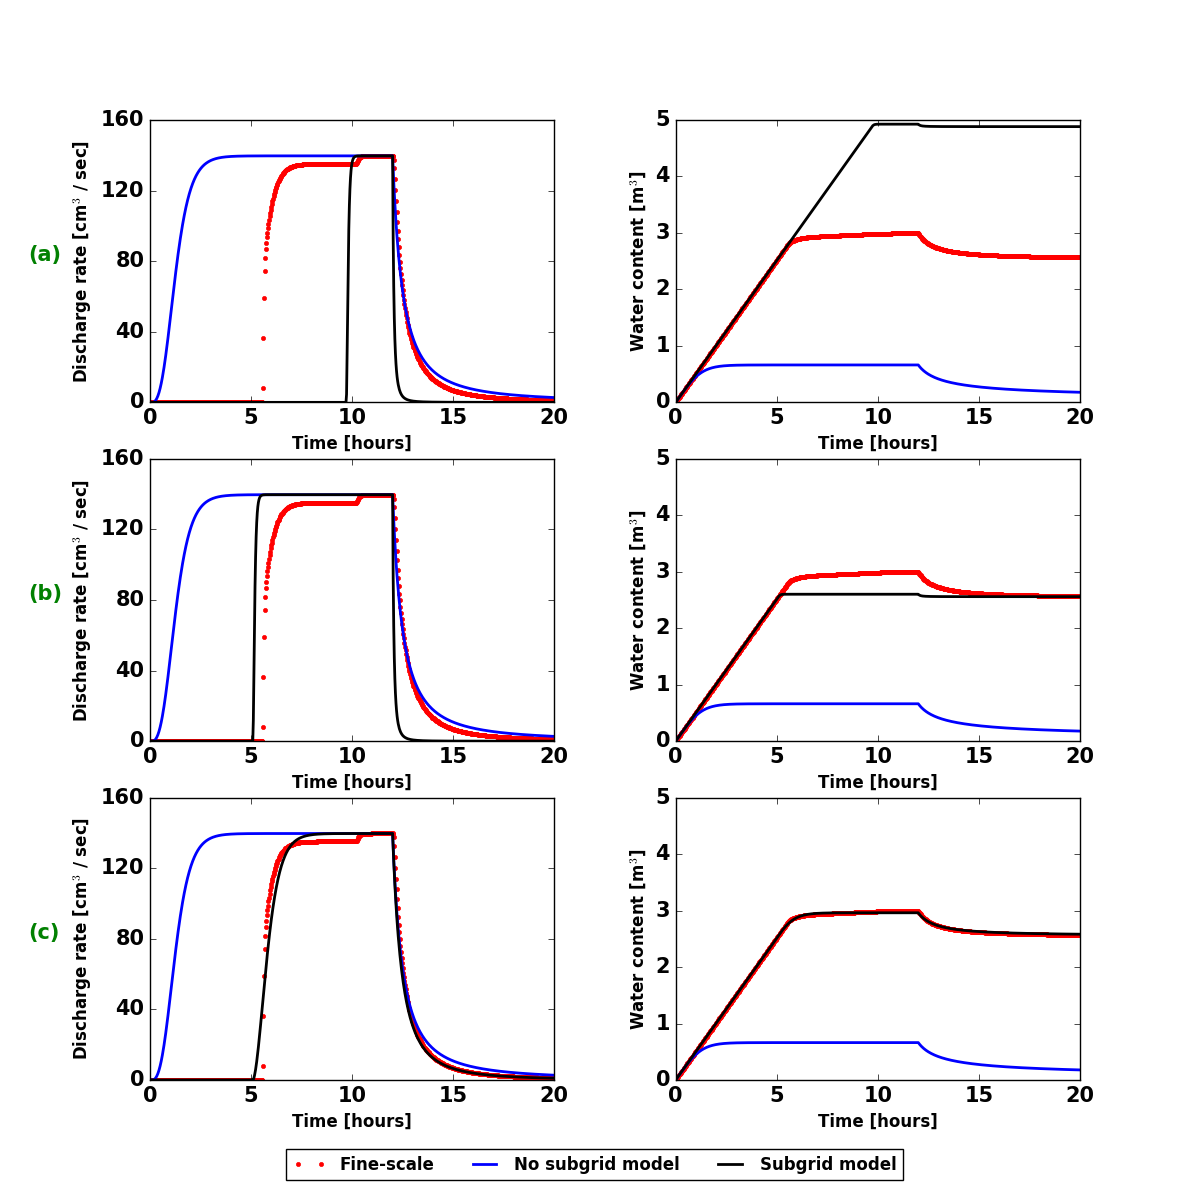
\includegraphics[width=13.cm, height=17.2cm]{./figures/new-model/POLYGON44-combined.png}
\caption{(Polygon C44) Comparison of the numerical results of the subgrid model with the fine-scale and no subgrid model results. Rows (top to bottom) correspond to Studies (I, II, and III(S$_2$)), (I, II, and III(S$_1$) with $\beta = 1.0$), and (I, II, and III(S$_1$) with $\beta = 3.0$), respectively.}
\label{polygon-C44}
\end{figure}

Figure~\ref{all-polygons-hydrographs} compares the hydrographs obtained in the simulations of the fine-scale and no-subgrid models to the results of Study III(S$_1$). These results correspond to polygons C06, C31, C40, C45, A01, and B01. Similar to the results of polygon C44, the high overland conductivity in the subgrid model is reduced by increasing the surface roughness (i.e., increasing $\beta$). It improves the shape of the hydrograph and replicates the rise and recession periods of the fine-scale simulations.
%The results of polygon A01 correspond to inlet$_2$ and outlet$_2$ boundaries, the results using inlet$_1$ and outlet$_1$ are discussed later. 
The water retained in the system in the subgrid, no-subgrid and fine-scale simulations are depicted in Figure~\ref{all-polygons-watercontent}. 
When the inlet boundary has obstructions (for example, polygon C06 in Figure~\ref{IWP-finemesh}) and divides the incoming water into different flow channels, the water reaches the outlet boundary at different times and lead to a dual-peak (or may be multiple-peak) hydrograph.  Due to only one grid cell in the subgrid model, the dual-peak behavior is not possible to capture.
Overall, the results of the subgrid model are very encouraging and consistently yield a better fit to the fine-scale results as compared to the no-subgrid model.
%
\begin{figure}
\centering
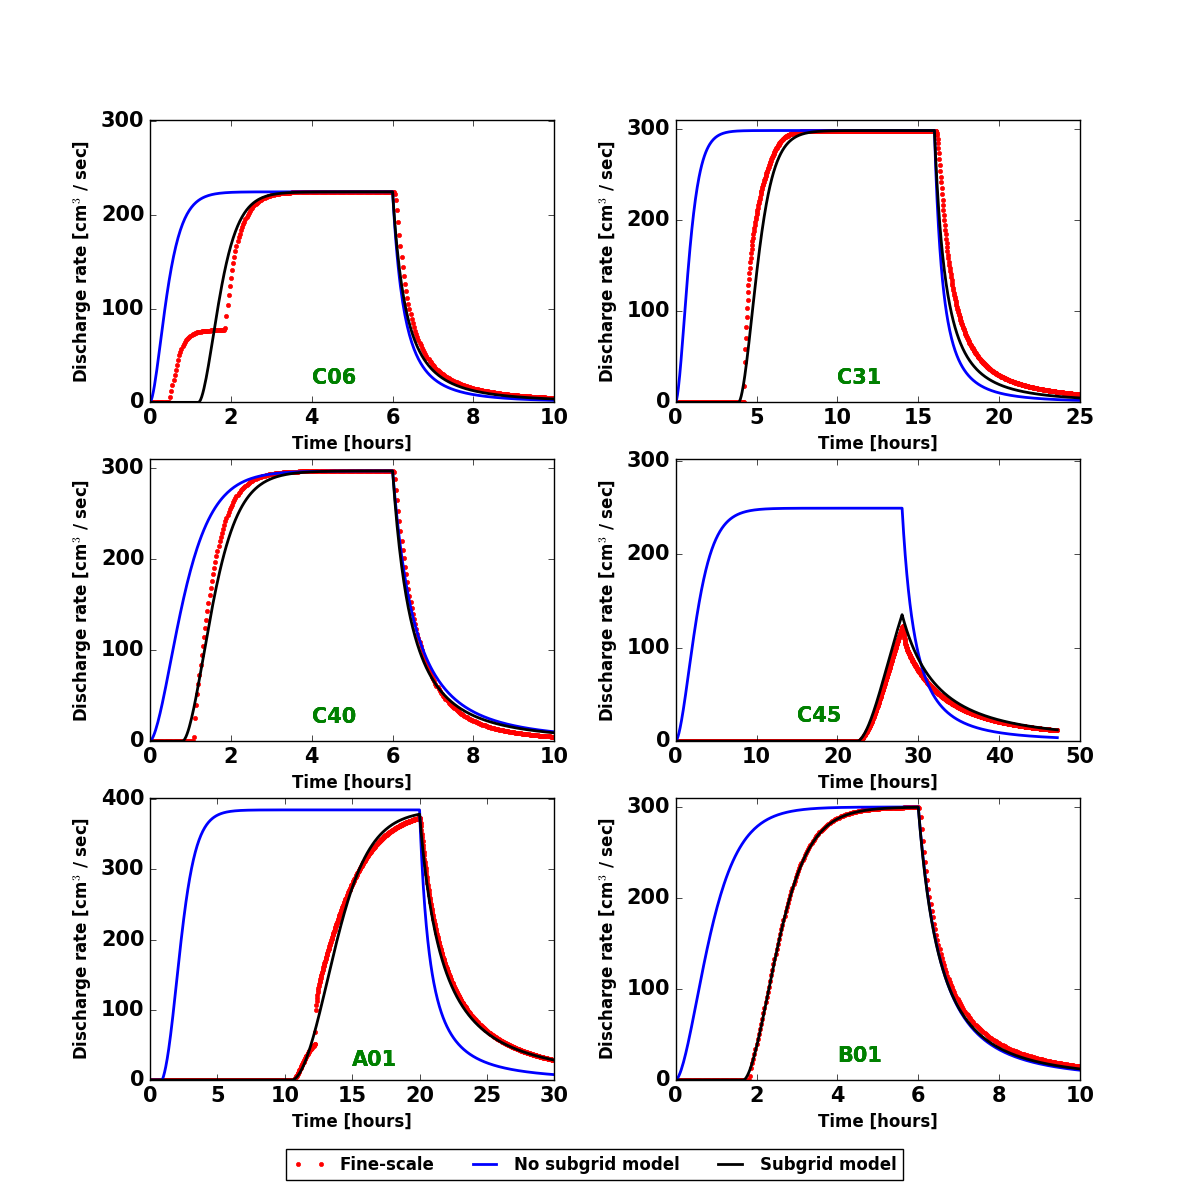
\includegraphics[width=13.2cm, height=17cm]{./figures/new-model/all-polygons-hydrograph.png}
%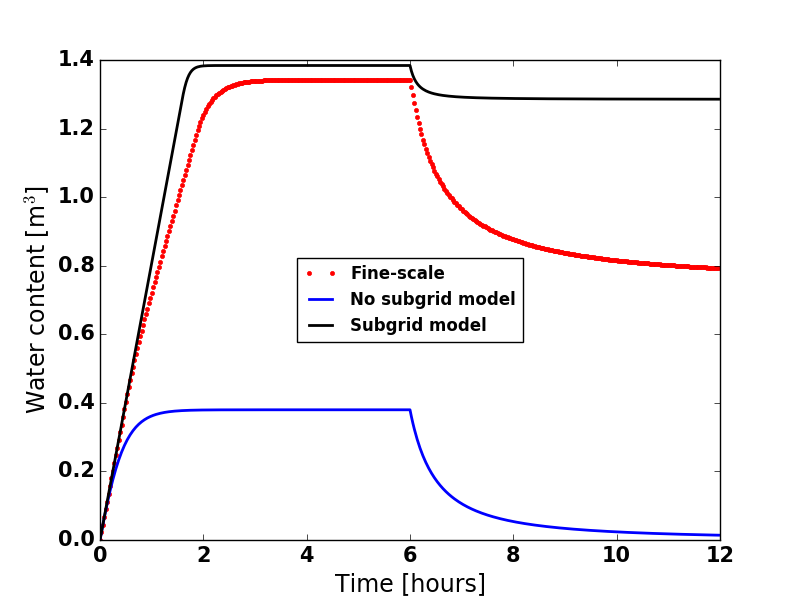
\includegraphics[width=6.2cm, height=6cm]{./figures/POLYGON06/POLYGON06watercontent.png}\\
%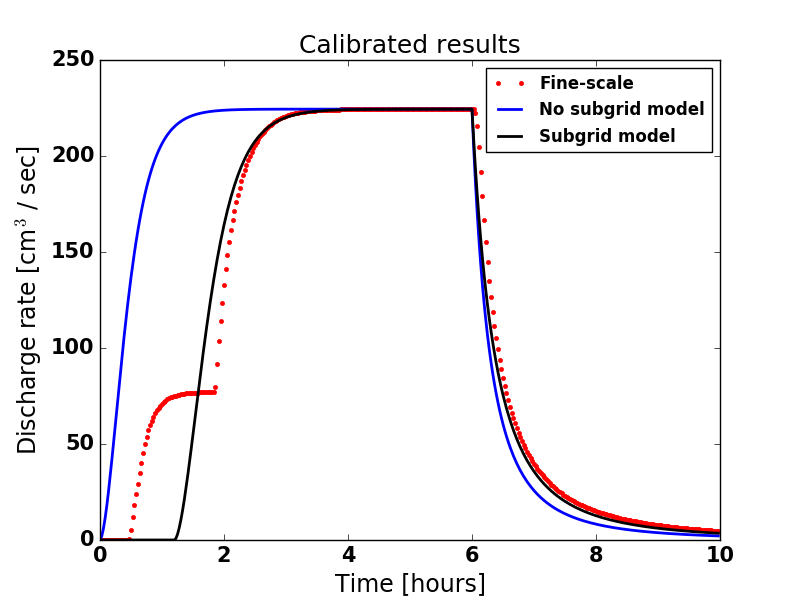
\includegraphics[width=6.2cm, height=6cm]{./figures/POLYGON06/POLYGON06dischargeCalibDDManning.png}
%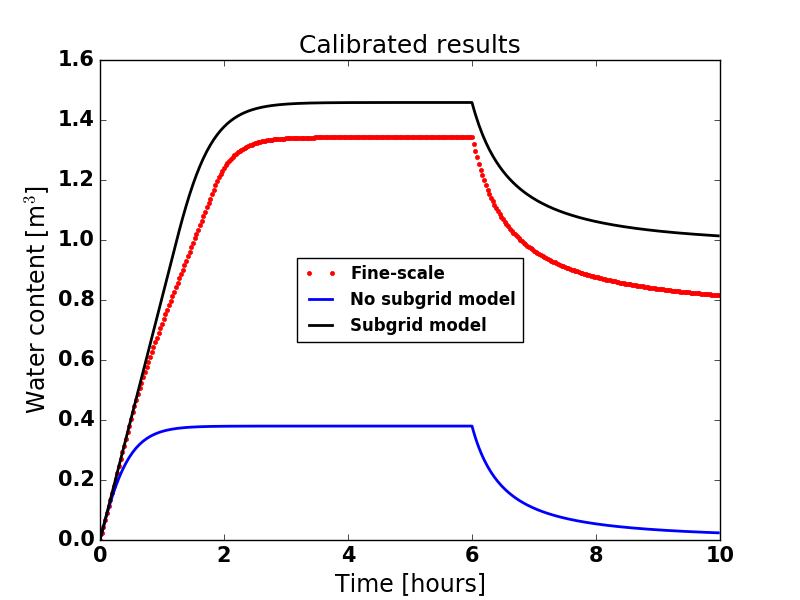
\includegraphics[width=6.2cm, height=6cm]{./figures/POLYGON06/POLYGON06watercontentCalibDDManning.png}
\caption{Comparison of hydrographs obtained in the subgrid, no-subgrid and fine-scale simulations for Study III(S$_1$) for the remaining six ice-wedge polygons (C06, C31, C40, C44, A0, and B01).}
\label{all-polygons-hydrographs}
\end{figure}

%
\begin{figure}
\centering
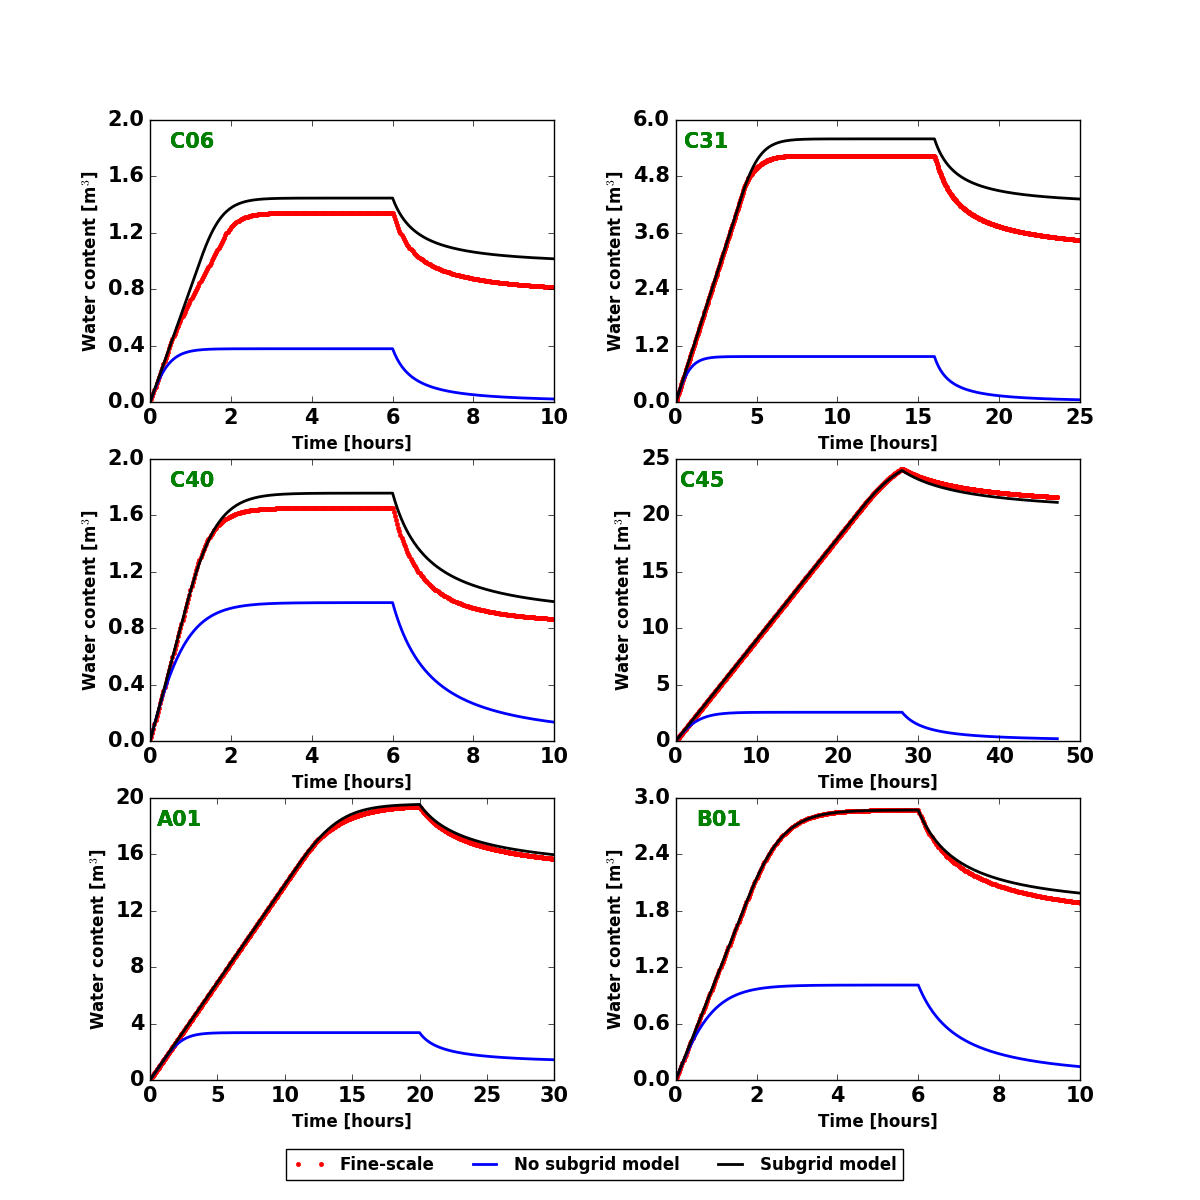
\includegraphics[width=13.2cm, height=17cm]{./figures/new-model/all-polygons-watercontent.png}
\caption{Comparison of total water content obtained in the subgrid, no-subgrid and fine-scale simulations for Study III(S$_1$) for the remaining six ice-wedge polygons (C06, C31, C40, C44, A0, and B01).}
\label{all-polygons-watercontent}
\end{figure}
%

The two variants (III(S$_1$) with $\beta =1 \, \text{and} \, 3$, and III(S$_2$)) of our subgrid model are equivalent in terms of form of the equations, but differ in how the subgrid parameters are determined. In Variant III(S$_2$), all the parameters are determined directly from the microtopography. While this variant generally improves the match to fine-scale simulations relative to the no-subgrid model, the calibration (Variant III(S$_1$)) of the depression depth and drag exponent are generally necessary to obtain a good fit. 

%
% Section: Results -- single IWP
% --------------------------------------------------------------------
\FloatBarrier
\subsection{Expanding from individual polygons to polygonal landscapes.}
%
An important question then is whether subgrid model parameters can be estimated semi-empirically from microtopography, thus avoiding calibration to fine-scale simulations.

Shown in Figure~\ref{curvefit-dd-manning} is calibrated depression depth versus uncalibrated depression depth.
The calibrated parameter is reasonably well-correlated to the uncalibrated depression depth, which is determined from geometric arguments (percolation algorithm).
The calibrated depression depth has a near-linear relationship with the uncalibrated depression depth (coefficient of variation of 0.82). 
%The drag factor varies between zero and one; as the depression depth decreases the drag factor goes to unity, representing flow over a flat surface. The fit indicates the resistance to flow increases with increasing depression depth. This finding is highly consistent with the discussion regarding the conductance terms in~\citet{panday2004fully}. 
The relatively good correlation in Figure~\ref{curvefit-dd-manning} suggests that fine-scale simulations may be avoided.
Instead, $\Delta_\text{exc}$ and $\Delta_\text{max}$ may be calculated directly from the univariant statistics of microtopography, while $\delta_\text{d}$ can be first estimated from microtopography by the percolation algorithm then used in the empirical fits of Figure~\ref{curvefit-dd-manning}.
%
\begin{figure}[!h]
\centering
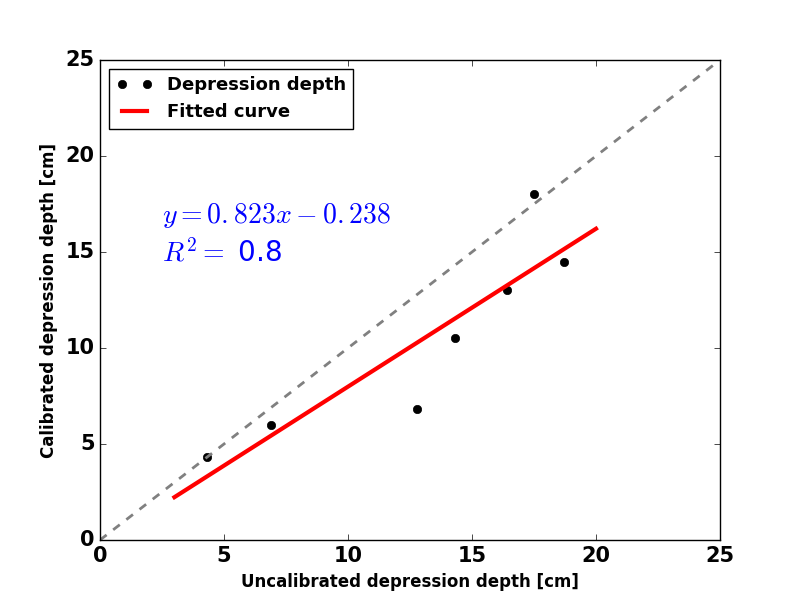
\includegraphics[width=11cm, height=7.5cm]{./figures/fittedcurve-dd-1.png}
%fittedcurve-manning-uncalibpd-2.png}
\caption{Linear fitted-curve to the depression depth data.}
\label{curvefit-dd-manning}
\end{figure}
%

An alternative strategy further limits the amount of algorithmic work that must be done on each individual polygon in a landscape.  
We consider a classification strategy for identifying depression depth and obstruction drag exponent that is based on the knowledge gained from the individual polygons.
We divide ice-wedge polygons into three types, high-centered, low-centered and intermediate-centered (a phase of transition from low-centered to high-centered) polygons. 
In this strategy, the classification compares the average trough vertex elevation $z_\text{avg}$ to the corresponding center elevation $z_\text{c}$:
%
\begin{itemize}
\item High-centered polygon : if $z_\text{c} - z_\text{avg} > 10$ cm
\item Low-centered polygon : if $z_\text{c} - z_\text{avg} < 0.0$ cm
\item Intermediate-centered polygon : if $ 0.0 \, \text{cm} <  z_\text{c} - z_\text{avg} \leq 10$ cm
\end{itemize}
%
The seven individual polygons calibrated above are classified as one low-centered, two intermediate, and four high-centered polygons, as seen in Figure \ref{beta-classification}'s $x$-axis.
The averaged subgrid parameters for each class are listed in Table~\ref{sg_par8a_classes}.
Note that $\Delta_\text{max}$ and $\Delta_\text{exc}$ are strongly correlated.
%
\begin{table}[!h]
\centering
\caption{Subgrid parameters for different types of polygons.}
\begin{tabular}{|p{2.cm}|p{2.5cm}|p{2.5cm}|p{2.5cm}|} 
%{|p{12.5mm}|p{7mm}|c|p{7mm}|p{7mm}|}
\hline
 & High-centered polygon & Low-centered polygon & Intermediate polygon \\ \hline
$\Delta_\text{max}(m)$ & 0.416 & 0.360 & 0.306  \\
$\delta_\text{d}(m)$ & 0.081 & 0.150 & 0.099 \\
$\Delta_\text{exc}(m)$ & 0.208 & 0.180 & 0.153  \\ \hline
\end{tabular}
\label{sg_para_classes}
\end{table}

Similarly, the parameter $\beta$ calibrates to how tortuous flow pathways are due to obstructions in flow through troughs.
For polygons with a flat-bottomed, well-established trough (independent of the polygon type), $\beta$ is close to 1.0.
As troughs become less flat-bottomed, and flow must go around and over obstructions in the troughs, $\beta$ must be increased to correctly predict effective flow rates.
In poorly established polygons, flow may overtop the rims and take extremely tortuous pathways, resulting in large $\beta$.
This characterization is shown in Figure \ref{beta-classification}'s $y$-axis.
%
\begin{figure}[!h]
\centering
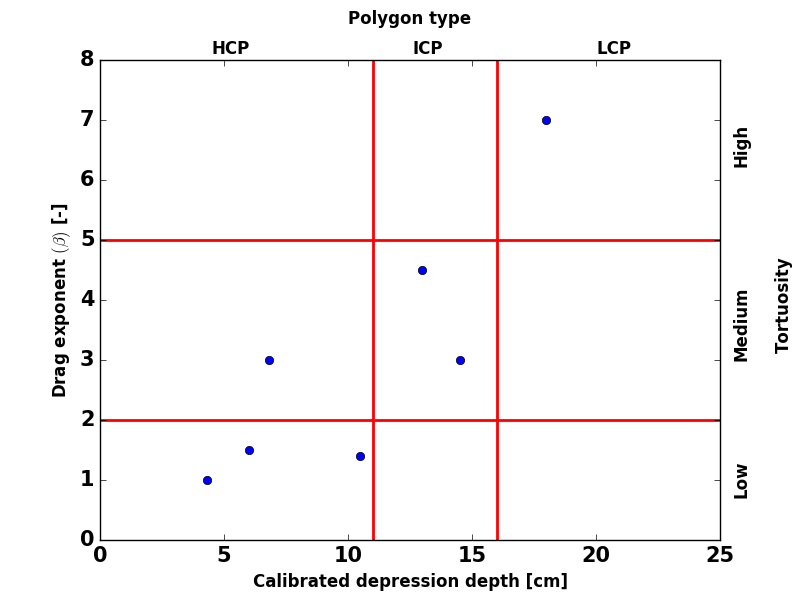
\includegraphics[width=11cm,height=7.5cm]
{./figures/new-model/beta-classification-3.png}
%fittedcurve-manning-uncalibpd-2.png}
\caption{The classifications in polygon type and tortuosity, and how they relate to $\delta_{\text{d}}$ and $\beta$ for the seven calibrated polygons.}
\label{beta-classification}
\end{figure}

Based on the results shown here, this procedure is expected to provide reasonably accurate representation of flow on a coarse mesh for the polygonal landscapes addressed here. 




%
% Section: Results -- cluster IWP
% --------------------------------------------------------------------
\FloatBarrier
\subsection{Results and Discussions: Cluster of ice-wedge polygons}\label{numerical-tests-cluster}
A cluster of polygons, (Figure~\ref{lobster-finemesh}) is taken from Area C, and consists of 21 polygons delineated by hand which have been determined through topography analysis to form a connected drainage unit.

Based on our definition above, polygons in the cluster of 21 polygons are either high-centered or intermediate-centered polygons.
In the evolution of low-centered polygon to high-centered polygon, the depression depth decreases due to the disappearance of the ridges. In the simulation study on 21 polygons cluster, each polygon is assigned values (subgrid parameters) based on its class.

We compare the hydrographs, cumulative discharge and total water content in the system for the simulations with the subgrid model to that of the fine-scale and no subgrid models in Figure~\ref{lobster-comparison-rainfall}. In each of the three simulations, a distributed water source representing snow melt was applied to the initally dry surface; water was allowed to flow out the lowest point on the boundary. 
The results with the subgrid model are greatly improved relative to the control without a subgrid model, when compared relative to the fine-scale results.
Simulation results with the no-subgrid model indicate more discharge and a drier surface.
This is a consequence of the ignored processes associated with microtopographic features (depressions and obstructions).
However, the simulated cumulative discharge obtained in the subgrid model shows the subgrid model follows the same trend as that of fine-scale simulation.
The retained water in the system due to microtopography is available for infiltration and/or evaporation but not runoff, which is critical to capture in integrated simulations.
The similarity in the hydrographs and water retention in the subgrid and fine-scale simulations provides confidence that the parameter's extraction approach adopted here is able to capture small-scale details in the coarsened models. Similar results were obtained (not shown) when we allowed water to run onto the domain from the upstream side of the perimeter instead of applying a distributed source.  

\begin{figure}[!h]
%\centering
\hskip -1.6cm  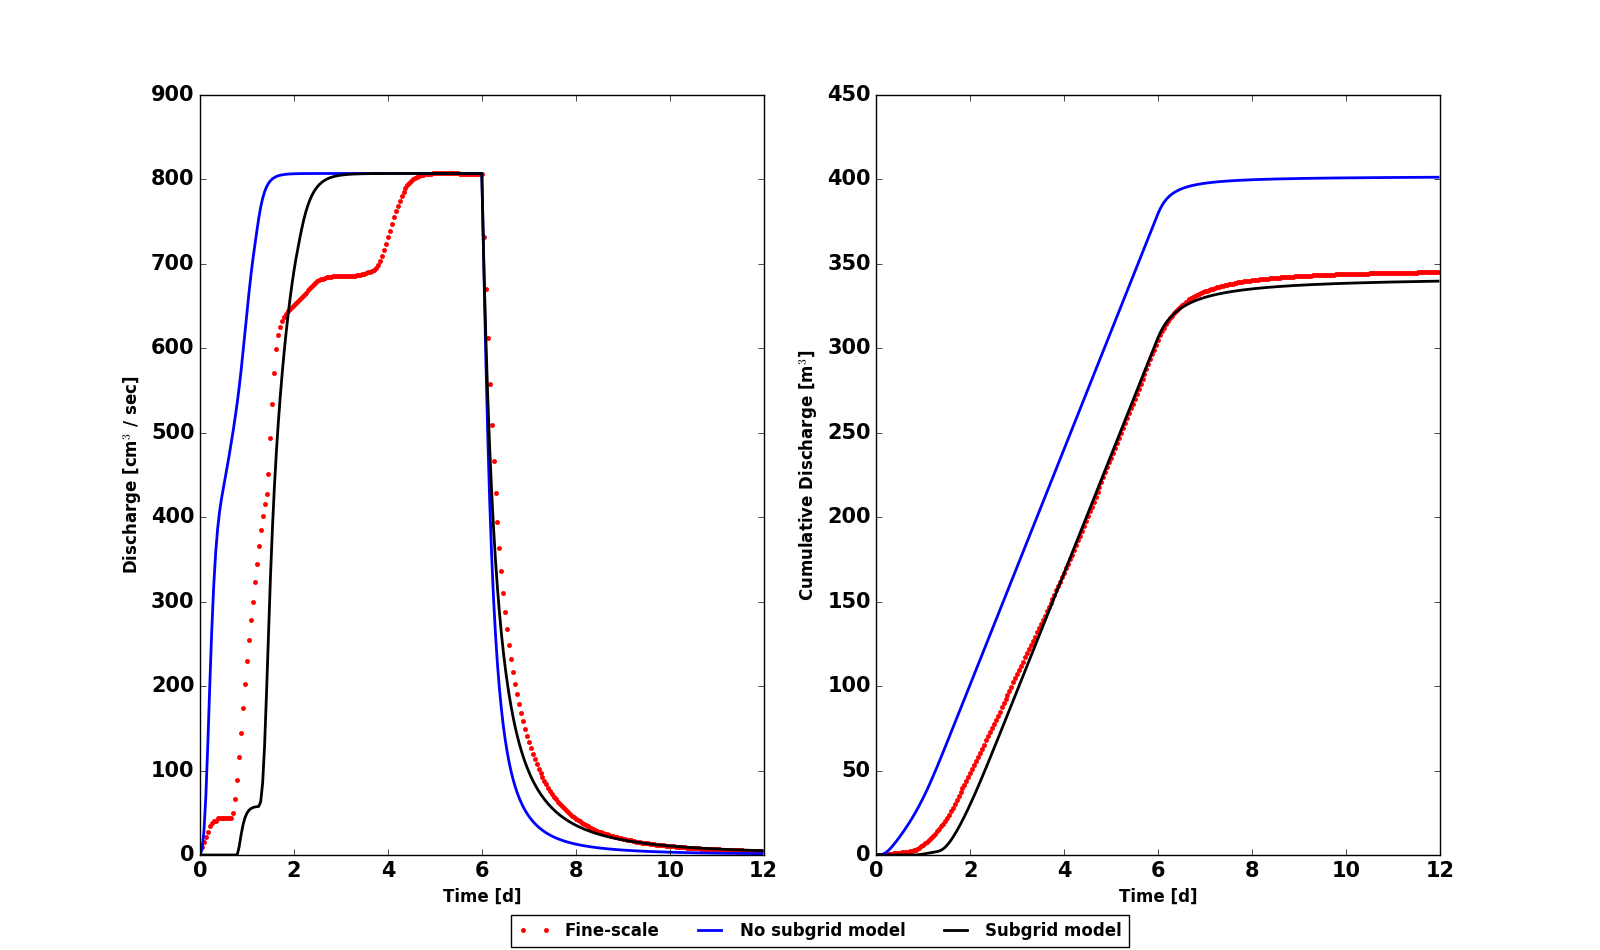
\includegraphics[width=15.cm, height=7.5cm]{./figures/new-model/discharge-Srun5SG_F.png} \\
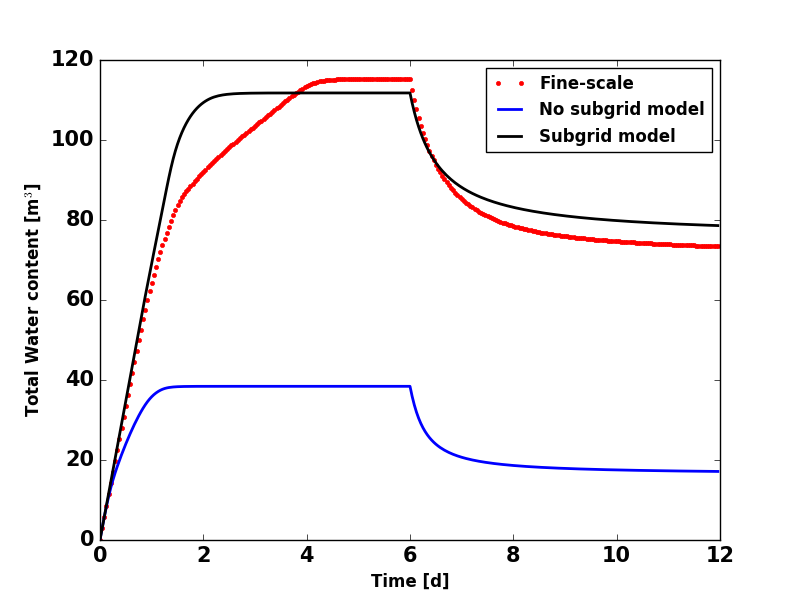
\includegraphics[width=10.cm, height=6.5cm]{./figures/new-model/Watercontent-Srun5SG_F.png}
\caption{Comparison of the hydrographs (top left), cumulative discharge (top right) and total water content (bottom row) in the system for three models on 21 polygons cluster. Subgrid parameters used in the simulation are listed in Table~\ref{sg_para_classes}. Effect of microtopography on the surface wetness is well represented by the subgrid model.}
\label{lobster-comparison-rainfall}
\end{figure}

\begin{figure}[!h]
\centering
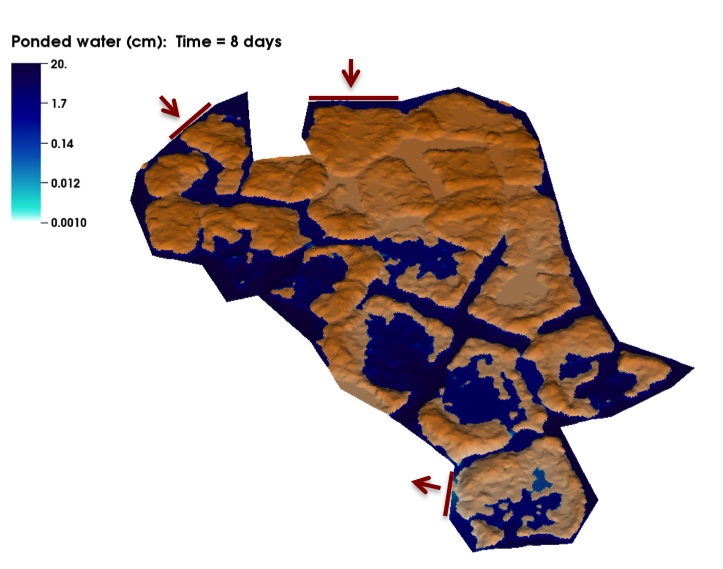
\includegraphics[width=6.cm, height=5.5cm]{./figures/new-model/finescale-pulsetest-8days-1.png}
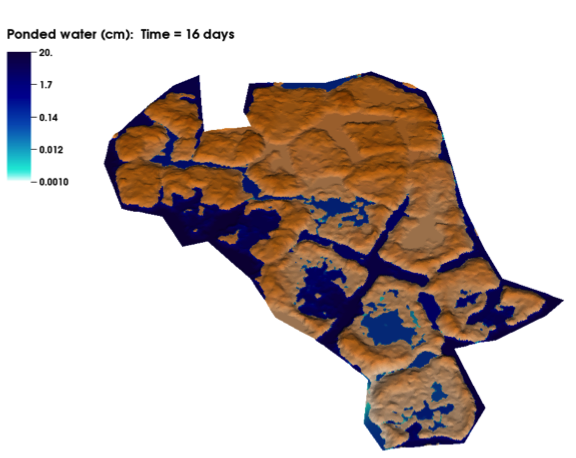
\includegraphics[width=6.cm, height=5.5cm]{./figures/new-model/finescale-pulsetest-16days-1.png}
\caption{An illustration of the fine-scale results on 21 polygons cluster. Inward and outward arrows indicate inlet and outlet boundaries. A pulse numerical test is performed with 8 days injection followed by 8 days recession. Snap shots taken at 8 day and 16 day.}
\label{lobster-pulsetest}
\end{figure}

%
% Section: Conclusions
% ================================================================================
\section{Conclusions}\label{conclusion}

The subgrid model presented in this paper is aimed at incorporating microtopographic effects in simulations of integrated surface/subsurface processes at the watershed-scale.
Standalone microtopography-resolving surface simulations are tractable with existing sophisticated computing tools.
However, a significant challenge is how to capture accurate flow behavior in watershed-scale integrated models because microtopography-resolving simulations of integrated models across watersheds are not feasible.
Seven ice-wedge polygons are considered to demonstrate that the effect of surface microtopography can be captured in coarsened models through the use of a subgrid model.
Numerical results of the subgrid model compare very well with the fine-scale simulations, depending on how the model parameters were estimated.
Our analysis shows that accurate estimate of depression depth is a determining factor for a close match between subgrid and fine-scale simulations.
Three different approaches for estimating the parameters for the subgrid representation were tested: (1) calibration of the depression depth from fine-scale simulations; (2) direct measurements from topography; (3) and classification-based parameterization.
Although calibration was necessary to obtain a good match, the calibrated parameters are correlated with parameters that can be estimated from microtopography alone, which suggests a tractable strategy for incorporating effects of microtopography without extensive fine-scale simulations. 
Finally, it has been demonstrated on a cluster of 21 polygons that a proper classification of polygons substantially improves predictions of runoff and surface water storage relative to coarse simulations without the subgrid model.
The subgrid model's ability to accurately capture fine-scale flow behavior provides confidence that a few parameters extracted from the available microtopographic data can be used to incorporate the fine-scale effects in watershed-scale integrated models.
%Integrated watershed-scale simulations with parameterized subgrid model using our recently developed mixed-dimensional model will be considered somewhere else.
%However, more research is needed to extend the approach developed here.
%For example, how to more accurately determine empirical relations for subgrid parameters to avoid any fine-scale simulations and calibration. 

\begin{comment}


\appendix
\section{Numerical Results}\label{appendix-A}
A simulation is performed to test the subgrid class-based parameterizaiton approach involving runoff only (no rainfall). Inlet and outlet boundaries are highlighted by the inward and outward arrow as shown in Figure~\ref{lobster-pulsetest}. The test consists of 8 days injection (steady state) at a constant rate followed by 8 days recession period (end of simulation). Figure~\ref{lobster-pulsetest} presents fine-scale simulation results. Mainly due to the high-centered and intermediate-centered polygons, a surface flow network is established in the interconnected troughs of polygons. To capture this type of flow behavior in the coarsened models, we compare simulated hydrographs (instantaneous discharge), cumulative discharge and the total water content obtained in fine-scale, subgrid and no-subgrid models in Figure~\ref{lobster-pulsetest-comparison}. Results indicate that the subgrid model improved the representation of microtopographic effects as compared to the no-subgrid model. A reasonable close match between the cumulative discharge and total water content in the fine-scale simulation and subgrid model is important for accurate representation of infiltration and evaporation processes. 
%The kinks in the fine-scale hydrographs are due to connecting different ponded areas to the main flow channel. 
Our numerical examples demonstrate that without altering the parameterization approach, different flow scenarios can accurately be simulated with the subgrid model.  
\begin{figure}[!h]
\centering
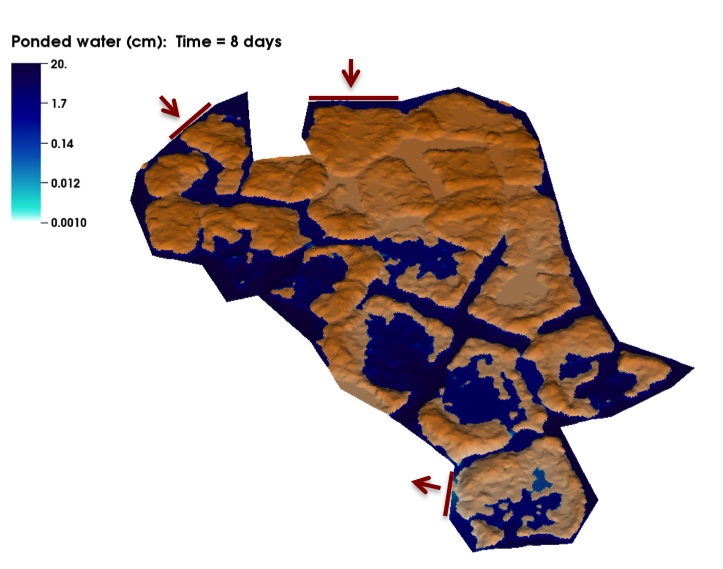
\includegraphics[width=6.cm, height=5.5cm]{./figures/new-model/finescale-pulsetest-8days-1.png}
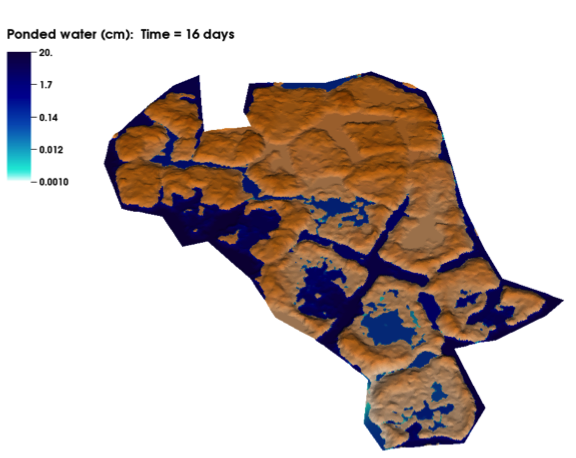
\includegraphics[width=6.cm, height=5.5cm]{./figures/new-model/finescale-pulsetest-16days-1.png}
\caption{An illustration of the fine-scale results on 21 polygons cluster. Inward and outward arrows indicate inlet and outlet boundaries. A pulse numerical test is performed with 8 days injection followed by 8 days recession. Snap shots taken at 8 day and 16 day.}
\label{lobster-pulsetest}
\end{figure}

\begin{figure}[!h]
%\centering
\hskip -1.6cm 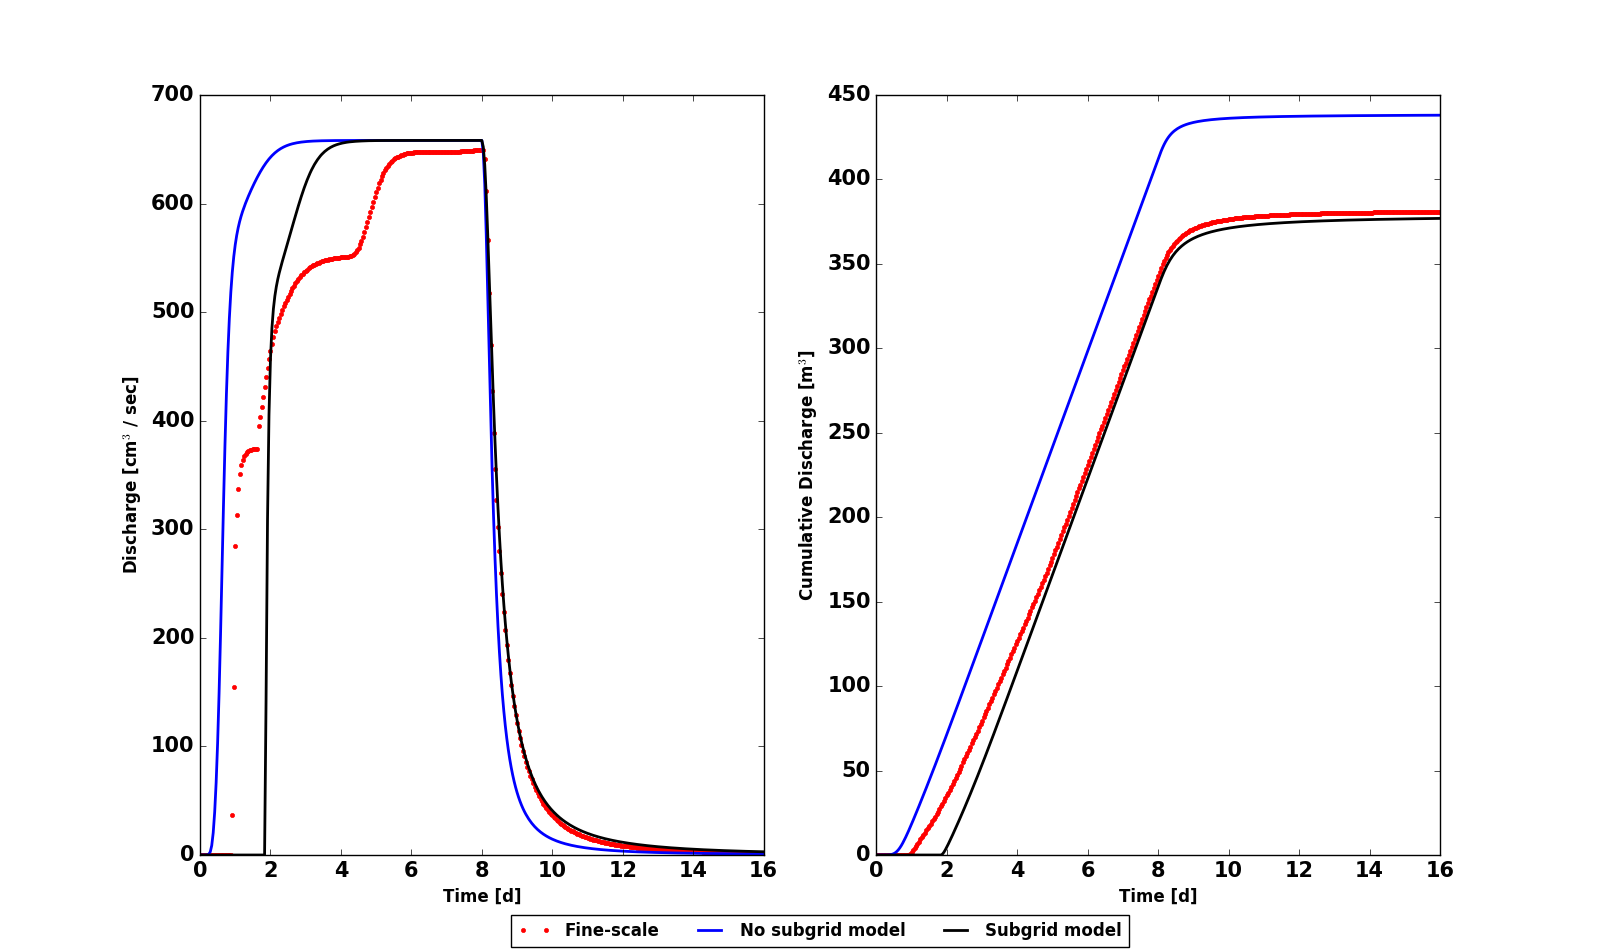
\includegraphics[width=15.cm, height=7.5cm]{./figures/new-model/discharge-sg_para_class_Srun4SG_A.png} \\

 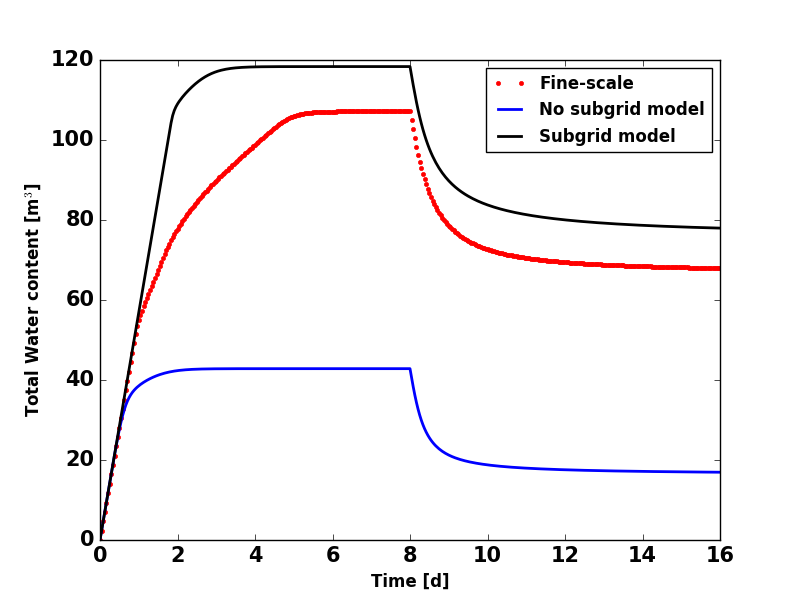
\includegraphics[width=10.cm, height=6.5cm]{./figures/new-model/Watercontent-sg_para_class_Srun4SG_A.png}
\caption{Results correspond to a pulse numerical test. Inlet and outlet boundaries are highlighted by arrows in Fig~\ref{lobster-pulsetest}. Comparison of the hydrographs (top left), cumulative discharge (top right) and total water content (bottom row) in the system for three models on 21 polygons cluster. Subgrid parameters used in the simulation are listed in Table~\ref{sg_para_classes}.}
\label{lobster-pulsetest-comparison}
\end{figure}
\end{comment}

\section*{Acknowledgments} 

 
\section*{References}

\bibliography{reference}

%% ------------------------------------------------------------------------ %%
\section*{Citations}

% Please use ONLY \citett and \citetp for reference citations.
% DO NOT use other cite commands (e.g., \citet, \citetyear, \nocite, \citetalp, etc.).

\subsection*{Cites made with \tt\string\citett\string{\string}}
...as shown by \citett{Boug10}, \citett{Buiz07}, \citett{Fra10},
\citett{Ghel00}, and \citett{Leit74}. 

\subsection*{Cites made with \tt\string\citetp\string{\string}}
...as shown by \citetp{Boug10}, \citetp{Buiz07}, \citetp{Fra10},
\citetp{Ghel00, Leit74}. 

...has been shown \citetp [e.g.,][]{Boug10,Buiz07,Fra10}.







%%%%%%%%%%%%%%%%%%%%%%%%%%%%%%%%%%%%%%%%%%%%%%%%%%%%%%%%%%%%%%%%
%
%  ACKNOWLEDGMENTS

\acknowledgments
This work was supported by Interoperable Design of Extreme-scale Application Software (IDEAS) project and by the Next Generation Ecosystem Experiment
(NGEE-Arctic) project. NGEE-Arctic is supported by the Office of Biological and Environmental Research in the DOE Office of Science. We are also grateful to Jitu Kumar and Terry Miller for help in constructing computational meshes.



%%  REFERENCE LIST AND TEXT CITATIONS
%
% Either type in your references using
%
% \begin{thebibliography}{}
% \bibitem{}
% Text
% \end{thebibliography}
%
% Or, to use BibTeX:
%
% Follow these steps
%
% 1. Type in \bibliography{<name of your .bib file>} 
%    Run LaTeX on your LaTeX file.
%
% 2. Run BiBTeX on your LaTeX file.
%
% 3. Open the new .bbl file containing the reference list and
%   copy all the contents into your LaTeX file here.
%
% 4. Run LaTeX on your new file which will produce the citations.
%
% AGU does not want a .bib or a .bbl file. Please copy in the contents of your .bbl file here.


\begin{thebibliography}{}

\bibitem[{\textit{Bell and Munoz}}(2008)]{Boug10} Bell, A.~H., and
Munoz, D.~P.  (2008). Activity in the superior colliculus reflects
dynamic interactions between voluntary and involuntary influences on
orienting behaviour. \textit{Eur. J. Neurosci.} 28, 1654--1660.

\bibitem[toth1962theory]{Toth, Jozsef}
{toth1962theory,
  title={A theory of groundwater motion in small drainage basins in central Alberta, Canada},
  author={Toth, Jozsef},
  journal={Journal of Geophysical Research},
  volume={67},
  number={11},
  pages={4375--4388},
  year={1962},
  publisher={Wiley Online Library}
}

@article{dunne1991effects,
  title={Effects of rainfall, vegetation, and microtopography on infiltration and runoff},
  author={Dunne, Thomas and Zhang, Weihua and Aubry, Brian F},
  journal={Water Resources Research},
  volume={27},
  number={9},
  pages={2271--2285},
  year={1991},
  publisher={Wiley Online Library}
}

@article{holden2005peatland,
  title={Peatland hydrology and carbon release: why small-scale process matters},
  author={Holden, Joseph},
  journal={Philosophical Transactions of the Royal Society of London A: Mathematical, Physical and Engineering Sciences},
  volume={363},
  number={1837},
  pages={2891--2913},
  year={2005},
  publisher={The Royal Society}
}
@article{kvaerner2008generation,
  title={Generation and regulation of summer runoff in a boreal flat fen},
  author={Kv{\ae}rner, Jens and Kl{\o}ve, Bj{\o}rn},
  journal={Journal of Hydrology},
  volume={360},
  number={1},
  pages={15--30},
  year={2008},
  publisher={Elsevier}
}

@article{huang2009influences,
  title={Influences of spatially heterogeneous roughness on flow hydrographs},
  author={Huang, Jen-Kuo and Lee, Kwan Tun},
  journal={Advances in water resources},
  volume={32},
  number={11},
  pages={1580--1587},
  year={2009},
  publisher={Elsevier}
}

@article{andresen2015disappearing,
  title={Disappearing Arctic tundra ponds: Fine-scale analysis of surface hydrology in drained thaw lake basins over a 65 year period (1948--2013)},
  author={Andresen, Christian G and Lougheed, Vanessa L},
  journal={Journal of Geophysical Research: Biogeosciences},
  volume={120},
  number={3},
  pages={466--479},
  year={2015},
  publisher={Wiley Online Library}
}

@article{bronstert1997modelling,
  title={Modelling of runoff generation and soil moisture dynamics for hillslopes and micro-catchments},
  author={Bronstert, Axel and Plate, Erich J},
  journal={Journal of Hydrology},
  volume={198},
  number={1},
  pages={177--195},
  year={1997},
  publisher={Elsevier}
}

@article{nakayama2006simulation,
  title={Simulation of spring snowmelt runoff by considering micro-topography and phase changes in soil layer},
  author={Nakayama, T and Watanabe, M},
  journal={Hydrology and Earth System Sciences Discussions},
  volume={3},
  number={4},
  pages={2101--2144},
  year={2006}
}

@article{jorgenson2001permafrost,
  title={Permafrost degradation and ecological changes associated with a warmingclimate in central Alaska},
  author={Jorgenson, M Torre and Racine, Charles H and Walters, James C and Osterkamp, Thomas E},
  journal={Climatic change},
  volume={48},
  number={4},
  pages={551--579},
  year={2001},
  publisher={Springer}
}

@article{liljedahl2016pan,
  title={Pan-Arctic ice-wedge degradation in warming permafrost and its influence on tundra hydrology},
  author={Liljedahl, Anna K and Boike, Julia and Daanen, Ronald P and Fedorov, Alexander N and Frost, Gerald V and Grosse, Guido and Hinzman, Larry D and Iijma, Yoshihiro and Jorgenson, Janet C and Matveyeva, Nadya and others},
  journal={Nature Geoscience},
  year={2016},
  publisher={Nature Publishing Group}
}

@article{lu2012modeling,
  title={Modeling methane emissions from the Alaskan Yukon River basin, 1986--2005, by coupling a large-scale hydrological model and a process-based methane model},
  author={Lu, Xiaoliang and Zhuang, Qianlai},
  journal={Journal of Geophysical Research: Biogeosciences},
  volume={117},
  number={G2},
  year={2012},
  publisher={Wiley Online Library}
}

@article{jan2017,
 title={An intermediate-scale model for thermal hydrology in low-relief permafrost-affected landscapes},
  author={Jan, Ahmad and Coon, Ethan T. and Painter, Scott L. and Garimella, Rao and Moulton, J. David},
  journal={Submitted to Computational Geosciences},
  year={2016},
}

@book{stammers1956effect,
  title={The effect of slope and microtopography on depression storage and surface detention},
  author={Stammers, William N and Ayers, HD},
  year={1956},
  publisher={publisher not identified}
}

@article{panday2004fully,
  title={A fully coupled physically-based spatially-distributed model for evaluating surface/subsurface flow},
  author={Panday, Sorab and Huyakorn, Peter S},
  journal={Advances in water Resources},
  volume={27},
  number={4},
  pages={361--382},
  year={2004},
  publisher={Elsevier}
}

@article{thompson2010role,
  title={Role of microtopography in rainfall-runoff partitioning: An analysis using idealized geometry},
  author={Thompson, Sally E and Katul, Gabriel G and Porporato, Amilcare},
  journal={Water Resources Research},
  volume={46},
  number={7},
  year={2010},
  publisher={Wiley Online Library}
}

@article{frei2012surface,
  title={Surface micro-topography causes hot spots of biogeochemical activity in wetland systems: A virtual modeling experiment},
  author={Frei, S and Knorr, KH and Peiffer, S and Fleckenstein, JH},
  journal={Journal of Geophysical Research: Biogeosciences},
  volume={117},
  number={G4},
  year={2012},
  publisher={Wiley Online Library}
}

@article{frei2014representing,
  title={Representing effects of micro-topography on runoff generation and sub-surface flow patterns by using superficial rill/depression storage height variations},
  author={Frei, S and Fleckenstein, Jan H},
  journal={Environmental Modelling \& Software},
  volume={52},
  pages={5--18},
  year={2014},
  publisher={Elsevier}
}

@article{schuur2015climate,
Author = {Schuur, E. A. G. and McGuire, A. D. and Schaedel, C. and Grosse, G. and
   Harden, J. W. and Hayes, D. J. and Hugelius, G. and Koven, C. D. and
   Kuhry, P. and Lawrence, D. M. and Natali, S. M. and Olefeldt, D. and
   Romanovsky, V. E. and Schaefer, K. and Turetsky, M. R. and Treat, C. C.
   and Vonk, J. E.},
Title = {{Climate change and the permafrost carbon feedback}},
Journal = {{NATURE}},
Year = {{2015}},
Volume = {{520}},
Number = {{7546}},
Pages = {{171-179}},
DOI = {{10.1038/nature14338}}
}


@Article{bg-11-6573-2014,
AUTHOR = {Hugelius, G. and Strauss, J. and Zubrzycki, S. and Harden, J. W. and Schuur, E. A. G. and Ping, C.-L. and Schirrmeister, L. and Grosse, G. and Michaelson, G. J. and Koven, C. D. and O'Donnell, J. A. and Elberling, B. and Mishra, U. and Camill, P. and Yu, Z. and Palmtag, J. and Kuhry, P.},
TITLE = {Estimated stocks of circumpolar permafrost carbon with quantified  uncertainty ranges and identified data gaps},
JOURNAL = {Biogeosciences},
VOLUME = {11},
YEAR = {2014},
NUMBER = {23},
PAGES = {6573--6593},
URL = {http://www.biogeosciences.net/11/6573/2014/},
DOI = {10.5194/bg-11-6573-2014}
}

@article{hinzman2005evidence,
  title={Evidence and implications of recent climate change in northern Alaska and other arctic regions},
  author={Hinzman, Larry D and Bettez, Neil D and Bolton, W Robert and Chapin, F Stuart and Dyurgerov, Mark B and Fastie, Chris L and Griffith, Brad and Hollister, Robert D and Hope, Allen and Huntington, Henry P and others},
  journal={Climatic Change},
  volume={72},
  number={3},
  pages={251--298},
  year={2005},
  publisher={Springer}
}

@article{lachenbruch1962mechanics,
  title={Mechanics of thermal contraction cracks and ice-wedge polygons in permafrost},
  author={Lachenbruch, Arthur H},
  journal={Geological Society of America Special Papers},
  volume={70},
  pages={1--66},
  year={1962},
  publisher={Geological Society of America}
}

@book{greene1963contraction,
  title={Contraction theory of ice-wedge polygons: A qualitative discussion},
  author={Greene, Gordon W},
  booktitle={Permafrost international conference: proceedings},
  pages={11--15},
  year={1963}
}

@article{mackay1990some,
  title={Some observations on the growth and deformation of epigenetic, syngenetic and anti-syngenetic ice wedges},
  author={Mackay, J Ross},
  journal={Permafrost and Periglacial Processes},
  volume={1},
  number={1},
  pages={15--29},
  year={1990},
  publisher={Wiley Online Library}
}


@article{mackay2004thermally,
  title={THERMALLY INDUCED MOVEMENTS IN ICE-WEDGE POLYGONS, WESTERN ARCTIC COAST},
  author={Mackay, JR},
  journal={Geomorphology: Critical Concepts in Geography},
  volume={5},
  number={1},
  pages={477},
  year={2004},
  publisher={Taylor \& Francis US}
}


@Article{kumar2016modeling,
AUTHOR = {Kumar, J. and Collier, N. and Bisht, G. and Mills, R. T. and Thornton, P. E. and Iversen, C. M. and Romanovsky, V.},
TITLE = {Modeling the spatiotemporal variability in subsurface thermal regimes across a low-relief polygonal tundra landscape},
JOURNAL = {The Cryosphere},
VOLUME = {10},
YEAR = {2016},
NUMBER = {5},
PAGES = {2241--2274},
URL = {http://www.the-cryosphere.net/10/2241/2016/},
DOI = {10.5194/tc-10-2241-2016}
}

@article{jorgenson2006abrupt,
  title={Abrupt increase in permafrost degradation in Arctic Alaska},
  author={Jorgenson, M Torre and Shur, Yuri L and Pullman, Erik R},
  journal={Geophysical Research Letters},
  volume={33},
  number={2},
  year={2006},
  publisher={Wiley Online Library}
}

@article {rowland2010arctic,
author = {Rowland, J. C. and Jones, C. E. and Altmann, G. and Bryan, R. and Crosby, B. T. and Hinzman, L. D. and Kane, D. L. and Lawrence, D. M. and Mancino, A. and Marsh, P. and McNamara, J. P. and Romanvosky, V. E. and Toniolo, H. and Travis, B. J. and Trochim, E. and Wilson, C. J. and Geernaert, G. L.},
title = {Arctic Landscapes in Transition: Responses to Thawing Permafrost},
journal = {Eos, Transactions American Geophysical Union},
volume = {91},
number = {26},
pages = {229--230},
year = {2010},
}

@inproceedings{liljedahl2012ice,
  title={Ice-wedge polygon type controls low-gradient watershed-scale hydrology},
  author={Liljedahl, AK and Hinzman, LD and Schulla, J{\"o}rg},
  booktitle={Proceedings of the Tenth International Conference on Permafrost},
  volume={1},
  pages={231--236},
  year={2012}
}


@article {spainter2016integrated, 
author = {Painter, Scott L. and Coon, Ethan T. and Atchley, Adam L. and Berndt, Markus and Garimella, Rao and Moulton, J. David and Svyatskiy, Daniil and Wilson, Cathy J.},
title = {Integrated surface/subsurface permafrost thermal hydrology: Model formulation and proof-of-concept simulations},
journal = {Water Resources Research},
volume = {52},
number = {8},
issn = {1944-7973},
url = {http://dx.doi.org/10.1002/2015WR018427},
doi = {10.1002/2015WR018427},
pages = {6062--6077},
keywords = {Permafrost, Active layer, Computational hydrology, permafrost, active layer, hydrology, simulations},
year = {2016},
}

@article{mwendera1992estimation,
  title={Estimation of depression storage and Manning's resistance coefficient from random roughness measurements},
  author={Mwendera, EJ and Feyen, J},
  journal={Geoderma},
  volume={52},
  number={3-4},
  pages={235--250},
  year={1992},
  publisher={Elsevier}
}

@Misc{ats-website, Author = "Ethan T. Coon", Title = "{ATS}: The {A}dvanced {T}errestrial {S}imulator", Note = "{h}ttp://github.com/amanzi/ats", Year = "2016" }


@Article{atchley2015,
AUTHOR = {Atchley, A. L. and Painter, S. L. and Harp, D. R. and Coon, E. T. and Wilson, C. J. and Liljedahl, A. K. and Romanovsky, V. E.},
TITLE = {Using field observations to inform thermal hydrology models of permafrost dynamics with ATS (v0.83)},
JOURNAL = {Geoscientific Model Development},
VOLUME = {8},
YEAR = {2015},
NUMBER = {9},
PAGES = {2701--2722},
URL = {http://www.geosci-model-dev.net/8/2701/2015/},
DOI = {10.5194/gmd-8-2701-2015}
}


@article{moulton2012high,
  title={High-level design of Amanzi, the multi-process high performance
computing simulator, Office of Environmental Management, United States Department
of Energy, Washington DC},
  author={Moulton, J David and Berndt, M and Garimella, R and Prichett-Sheats, L and Hammond, G and Day, M and Meza, J.C.},
  journal={},
  volume={},
  number={},
  year={2012},
  publisher={Wiley Online Library}
}


@article{ecoon2016managing,
  title={Managing complexity in simulations of land surface and near-surface processes},
  author={Coon, Ethan T and Moulton, J David and Painter, Scott L},
  journal={Water Resources Research},
  volume={78},
  pages={134--149},
  year={2016},
  publisher={Elsevier}
}

@article{Skurikhin2013,
author = {Alexei N. Skurikhin and Chandana Gangodagamage and Joel C. Rowland and Cathy J. Wilson},
title = {Arctic tundra ice-wedge landscape characterization by active contours without edges and structural analysis using high-resolution satellite imagery},
journal = {Remote Sensing Letters},
volume = {4},
number = {11},
pages = {1077-1086},
year = {2013},
doi = {10.1080/2150704X.2013.840404}

}


\end{thebibliography}


\end{document}




